\documentclass [11pt, proquest] {uwthesis}[03/03/15] %[2021/06/15]
\usepackage{graphicx}
\usepackage[sort&compress,numbers]{natbib}
\usepackage{multirow}
\usepackage{caption}
\usepackage{subcaption}
\usepackage[breaklinks,hidelinks]{hyperref}
\usepackage{amsmath,amssymb,amsfonts,amsthm,epsfig,epstopdf,titling,url}
\usepackage{enumerate}
\usepackage{algorithm,algorithmic}
\usepackage{{booktabs}}
\usepackage[numbers]{natbib}
\newenvironment{packed_enum}{
\begin{enumerate}[a)]
  \setlength{\itemsep}{1pt}
  \setlength{\parskip}{0pt}
  \setlength{\parsep}{0pt}
}{\end{enumerate}}

\newenvironment{packed_enum1}{
\begin{enumerate}[1.]
  \setlength{\itemsep}{1pt}
  \setlength{\parskip}{0pt}
  \setlength{\parsep}{0pt}
}{\end{enumerate}}

\newenvironment{packed_enum_par}{
\begin{enumerate}[1)]
  \setlength{\itemsep}{1pt}
  \setlength{\parskip}{0pt}
  \setlength{\parsep}{0pt}
}{\end{enumerate}}

\newenvironment{packed_e}{
\begin{enumerate}
  \setlength{\itemsep}{1pt}
  \setlength{\parskip}{0pt}
  \setlength{\parsep}{0pt}
}{\end{enumerate}}

\newenvironment{packed_itemize}{
\begin{itemize}
  \setlength{\itemsep}{1pt}
  \setlength{\parskip}{0pt}
  \setlength{\parsep}{0pt}
}{\end{itemize}}

% ==========   Local defs and mods

% ----------- definitions format
\theoremstyle{definition}
\newtheorem{defn}{Definition}
\newtheorem{conj}{Conjecture}[section]
\newtheorem{exmp}{Example}[section]



% ================================
% DOCUMENT
% ================================
\begin{document}

\prelimpages
% \raggedbottom


% ---------------------------

\Title{Project TLDR: Standalone desktop application for question answering and summarization using resource-efficient LLMs}

\Author{Manu Hegde}
\Year{2025}
\Program{Computer Science and Software Engineering}

\Chair{Erika Parsons}{}{School of Science, Technology, Engineering \& Mathematics}
\Signature{Michael Stiber}
\Signature{Shane Steinert-Threlkeld}

\copyrightpage

\titlepage  


\setcounter{page}{-1}
\abstract{

This project presents the design and development of a standalone desktop application that enables offline question answering and summarization over a user-provided document corpus using resource-efficient large language models (LLMs). Targeted to run on Apple's M1 / M2 hardware, it leverages on-device processing through Apple's neural engine (ANE) and Apple metal shaders (GPU). The application aims to address growing concerns about data privacy, resource consumption, and user accessibility. Unlike cloud-based tools, which require constant internet connectivity and expose sensitive data to third-party servers, this application provides a secure, localized alternative optimized for academic researchers and students. Core capabilities include a graphical interface and retrieval-augmented generation (RAG) over user specified corpus, while leveraging only a fraction of system resources to allow for seamless multi-tasking. Evaluation is based on both functional quality (e.g., BERTScore comparison to ChatGPT) and nonfunctional metrics (e.g., memory, CPU usage). The outcome is a practical and efficient tool that allows users to interact with large academic corpora while maintaining system responsiveness and data confidentiality.


}

%
% ----- contents & etc.
%
\tableofcontents
\listoffigures
\listoftables  

%
% ----- acknowledgments
%
\acknowledgments{% \vskip2pc
  % {\narrower\noindent
I would like to express my gratitude to Prof. Erika Parsons for all the valuable guidance and help during this work. Furthermore, I sincerely thank Prof. Steinert-Threlkeld and Prof. Stiber for accepting my request to be on the committee for this thesis and for providing precise feedback.
  % \par}
}
%
% end of the preliminary pages
 
 
 
%
% ==========      Text pages
%
\textpages
% ============================================================
%
%                   CHAPTER 1: INTRODUCTION
%
% =============================================================

\chapter {Introduction}
\label{ch:Introduction}

%----------------------
\section{Background and Motivation}
\label{sec:Background and Motivation}
%----------------------
The increasing volume of academic and research materials necessitates the development of efficient tools capable of processing and interpreting large text corpus \cite{vaswani2017attention, devlin2018bert}. Students and researchers, identified as the primary intended users of this project, frequently interact with numerous papers and books, requiring methods to both understand individual documents and handle collections of documents in a single context for a holistic understanding of subjects or topics \cite{liu2019text}.

Existing tools often require significant manual intervention, particularly when more than one document is involved \cite{beltagy2020longformer}.

Furthermore, many current solutions, such as popular online Large Language Models (LLMs) like ChatGPT, Gemini, and Claude, compel users to share potentially sensitive data with third-party servers. This practice raises considerable concerns regarding \textbf{privacy and data security} \cite{bommasani2021opportunities, wolf2019huggingface}. For example, if a researcher needs a summary of survey data, the data needs to be shared with the online tool. Reported instances of leakage of data shared with ChatGPT exacerbate these concerns \cite{openai2023gpt4}. Additionally, online LLMs may include information from \textbf{unknown sources} in their output, leading to loss of credibility of the information.

While desktop-based solutions like Ollama and LLamaFile do exist, their goals are intended towards enabling a large number of open-source models to run on a diverse set of hardware \cite{touvron2023llama}. This narrows their user base to only those who are \textbf{technically skilled}. Furthermore, it limits their scope to optimize performance and streamline usability for specific use cases. These solutions also do not provide the ability to perform Question-Answering over multiple documents \cite{izacard2021leveraging}.

This project is motivated by the \textbf{need for a convenient, confidential, and productivity-enhancing tool designed specifically for students and researchers}, providing secure, local, and resource-efficient capabilities for interacting with their document collections. It aims to fill the gap in the current set of tools for researching information by leveraging the latest advancements in Natural Language Processing \cite{brown2020language, raffel2020exploring}.
%----------------------
\section{Research Objective and Solution}
\label{sec:ResearchObjectiveandSolution}
%----------------------
This research aims to employ Deep Learning (DL) methods to create Computational Fluid Dynamics (CFD) simulations involving the interaction of fluid flow with an obstacle in a 2-dimensional environment. The objective is to decrease the simulation's execution time compared to conventional simulation techniques. To achieve this goal, a novel neural network architecture incorporating approaches from existing research in DL for CFD and new ideas for this field are proposed. The DL solution proposed is an end-to-end data-driven solution. This means it is a unified process that can use data to learn the complexities of a fluid flow spatial structure's evolution over time. It can also quickly adapt to changing environments represented by different datasets by directly learning from raw data that represents the intrinsic patterns of fluid mechanics. This solution combines an autoencoder and a generator implemented with a ConvLSTM neural network.

Compared to related solutions in DL for CFD that use different datasets (like Homogeneous Isotropic Turbulence data) or focus on the Dimensionality Reduction techniques of the input data, this research's emphasis is on generating a fluid flow simulation interacting with an obstacle and how well it generalize between distinct shapes of obstacles in various positions and sizes. Additionally, this research studies the effectiveness of the Convolutional LSTM neural network by implementing the model using only this type of architecture.

Two primary metrics are used to evaluate the success of this solution: execution time and accuracy. The execution time of the simulation using the DL model is compared to a traditional CFD simulation. Its accuracy, when compared to the conventional method, is measured using the Mean Squared Error (MSE) (See Equation~\ref{eq:mse}), also known as the Mean Squared Deviation (MSD). The goal is to reduce the execution time while maintaining a good enough accuracy to preserve the pattern structure of the fluid in the generated sequence flow.

\begin{equation}
    \begin{aligned}
        MSE(y, \hat{y}) = \frac{1}{n} \sum_{i=1}^{n}(y_i-\hat{y_i})^2
    \end{aligned}
    \label{eq:mse}
\end{equation}

%----------------------
\section{Scope}
\label{sec:Scope}
%----------------------
The proposed solution focuses on the simple case of a fluid flow interacting with a stationary shape in a 2-dimensional environment and replicates the fluid's behavior using a DL model as accurately as possible while improving the execution time compared to a traditional simulation. 

Because the Navier-Stokes equations used in fluid dynamics are so complex and chaotic (See Section~\ref{ch:TheoreticalBackground}), finding an analytical solution for some problems is impossible. This is why numerical techniques are used to approximate the solutions. Research and industry rely on approximated results to perform their experiments and designs. This means that even when the model solution results are not so precise but provide a fast approximation of the data, it still has value since it is a tool to quickly iterate initial designs that can later be validated with more accurate but slow and resource-demanding methods.

%----------------------
\section{Paper overview}
\label{sec:PaperOverview}
%----------------------
This paper is organized as follows: Chapter~\ref{ch:TheoreticalBackground} explains the main concepts for this work related to Computational Fluid Dynamics and Deep Learning. Chapter~\ref{ch:RelatedWork} presents related work and the current state of DL research for CFD and discusses previous related research relevant to this study. Chapter~\ref{ch:Methods} explains all the methods involved in developing this research and the solution, including the data collection, the DL model architecture and training, and the evaluation techniques. Chapter~\ref{ch:Results} shows the results with its analysis and discussion. Finally, Chapter~\ref{ch:Conclusion} presents the conclusions of this research, its limitations, and future work based on the results obtained.



% ============================================================
%
%                   CHAPTER 2: THEORETICAL BACKGROUND
%
% =============================================================

\chapter {Theoretical Background}
\label{ch:TheoreticalBackground}

This chapter provides the theoretical foundation for the key concepts relevant to the design and implementation of this project. It focuses on topics related to Large Language Models (LLMs) and the architectural characteristics of Apple Silicon (M1/M2). The sections that follow explore essential components of LLM inference, the unique hardware features of Apple Silicon, and optimizations leveraged to enable efficient on-device performance.

%----------------------
\section{Large Language Models and Inference Components}
\label{sec:LargeLanguageModelsAndInferenceComponents} 
%----------------------

Large Language Models (LLMs) are transformer-based neural networks trained on massive text corpora to generate text in human language. They can mimic human-like conversations, storytelling, and can respond to abstract instructions. These models, such as GPT, LLaMA, and Falcon, rely on the transformer architecture introduced by Vaswani et al.~\cite{vaswani2017attention}, where self-attention mechanisms enable the model to capture dependencies across different parts of the input sequence (as seen in Figure ~\ref{fig:transformer_architecture}). Inference in LLMs involves several critical components, each contributing to performance, quality, and resource efficiency.

\begin{figure}[h]
    \centering
    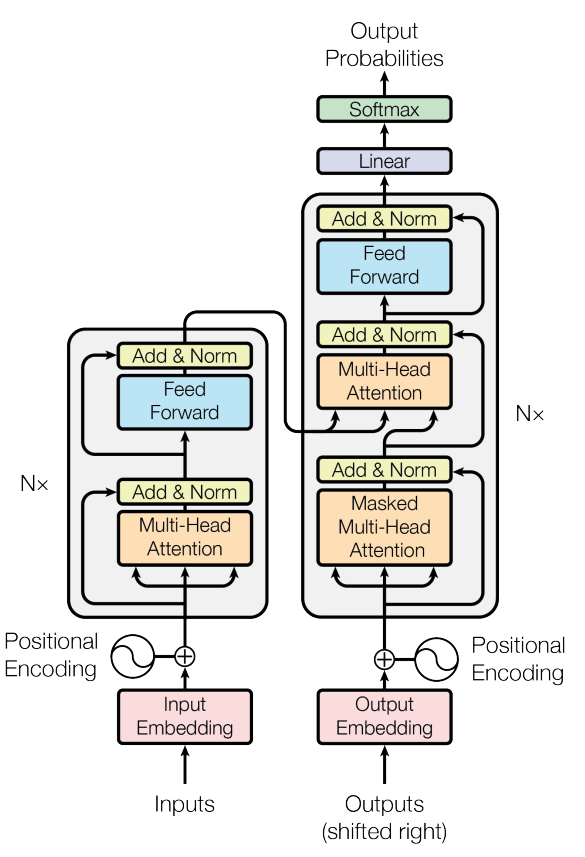
\includegraphics[width=0.4\linewidth]{images/transformer-architecture.png}
    \caption{Transformer architecture ~\cite{vaswani2017attention}}
    \label{fig:transformer_architecture}
\end{figure}
At the core of LLM inference lies the \textbf{context window}, which denotes the maximum number of tokens the model can attend to at any given time. A token is a piece of input, ranging from a subword to even a phrase, depending on the tokenization scheme of the model. For models like LLaMA-2, the context window can be up to 4,096 or 8,192 tokens~\cite{touvron2023llama}. During inference, the model builds an internal representation of this input context, which is used to generate predictions for the next token.

\begin{figure}[h]
    \centering
    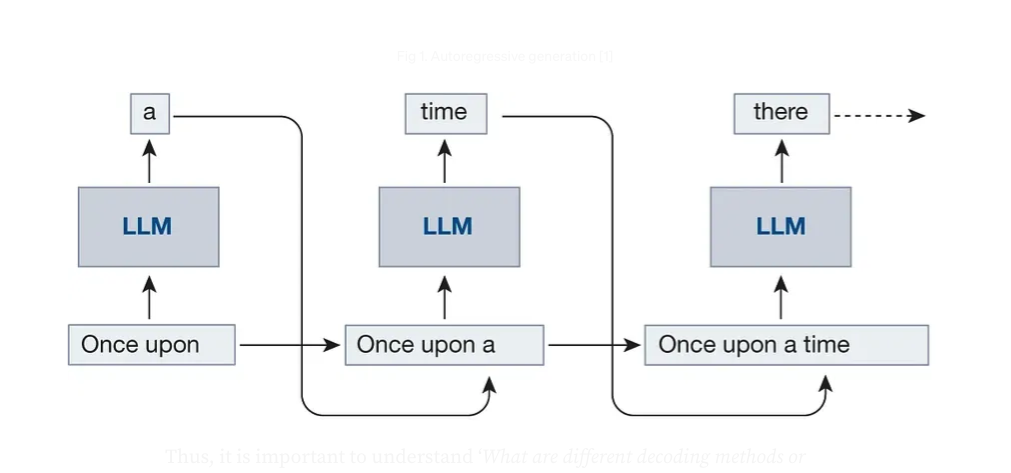
\includegraphics[width=0.6\linewidth]{images/autoregressive-decoding.png}
    \caption{Autoregressive decoding ~\cite{nabi2024all}}
    \label{fig:autoregressive_decoding}
\end{figure}

The \textbf{Key-Value (KV) cache} is a performance optimization central to LLM performance. During autoregressive decoding for text generation, a Large Language Model (LLM) processes the entire input sequence to generate a single output token. This newly generated token is then appended to the sequence, and the model repeats the process iteratively (as seen in Figure ~\ref{fig:autoregressive_decoding}). However, this leads to redundant computation over previously processed tokens at each step. To mitigate this inefficiency, the \textit{key} and \textit{value} vectors computed during the attention mechanism of the transformer can be cached. This \textit{KV caching} technique significantly reduces repeated computation by reusing the stored attention states from prior steps, thereby improving inference speed and memory efficiency. These cached representations allow the model to efficiently attend to all previously generated tokens without recalculating the entire attention graph ~\cite{alammar2018illustrated}. This caching mechanism reduces computational overhead and is especially vital when running LLMs on resource-constrained devices.

Furthermore, the token generation is governed by a sampling algorithm, which yields the output token by sampling on the output probability distribution obtained from the model. Common strategies include greedy sampling, top-$k$ sampling and temperature scaling. A \textbf{token sampler} module is responsible for leveraging these strategies to generate the output token. This can be a resource-hungry step, since this involves processing the probability distribution over the entire vocabulary of the model.

Therefore, the core components required for consistent text generation in an LLM-based system include the model weights, the LLM context (comprising the KV cache and vocabulary), and the token sampler.

Finally, the inference engine managing the model (e.g., llama.cpp, Hugging Face Transformers, or Apple CoreML) orchestrates the context construction, efficient memory handling of the KV cache, and optimized computation for each transformer layer, accounting for quantization if any. These components together define the responsiveness, accuracy, and resource efficiency of the LLM in real-time applications.

%----------------------
\section{LLM Weight Quantization}
\label{sec:LLMWeightQuantization} 
%----------------------
Quantization is a model weight compression technique that reduces the precision of the numbers used for representing model parameters. Typically, reducing the precision from 32-bit floating point to lower-bit integers such as 8-bit, 4-bit, or even 3-bit values. This significantly decreases memory usage and computational requirements, making it possible to run large language models (LLMs) efficiently on edge devices or in real-time environments without sacrificing too much accuracy \cite{jacob2017quantization,hubara2016quantized}.

Within the \texttt{ggml} framework and its application in \texttt{llama.cpp} \cite{llamacpp2023}, various quantization schemes have been introduced to significantly reduce the size and memory footprint of LLM weights. One such scheme is \texttt{Q3\_K\_L}, a 3-bit quantization format specifically designed to balance compression efficiency and model performance \cite{talamdupula2024guide,li2024quantization}. In \texttt{Q3\_K\_L}, weights are grouped in sets of 256 and quantized with shared scaling factors, offset by a zero-point, enabling fine-grained approximation while preserving hardware efficiency. Notably, \texttt{Q3\_K\_L} makes use of 4-bit storage for each quantized value (3 bits for the quantized magnitude and 1 extra bit for improved alignment and bit-packing efficiency), along with 8-bit scales and 6-bit zero-points per group. This layout ensures better alignment with SIMD instructions and allows for faster matrix-vector multiplications, which are critical during transformer inference \cite{pope2022efficiently}. ~\ref{tab:quantization-comparison} shows the comparison between common quantization schemes used in GGML. While this format slightly increases decoding complexity compared to simpler formats like \texttt{Q4\_0}, it provides a favorable tradeoff between model accuracy and size, especially for models deployed in edge or offline settings \cite{ollama2023,llamafile2023}.
Therefore, this project primarily employs model weights quantized using the \texttt{Q3\_K\_L} scheme.

\begin{table}[h]
\centering
\caption{Comparison of Common Quantization Formats in \texttt{ggml}/\texttt{llama.cpp}}
\label{tab:quantization-comparison}
\begin{tabular}{|l|c|c|c|c|}
\hline
\textbf{Format} & \textbf{Bits/Weight} & \textbf{Group Size} & \textbf{Remarks} \\ \hline
Q4\_0     & 4 bits   & 32 weights          & Baseline 4-bit scheme \\ \hline
Q4\_K     & 4 bits   & 64 weights    & Better accuracy than Q4\_0 \\ \hline
Q5\_K     & 5 bits   & 64 weights           & Higher accuracy, more storage \\ \hline
Q8\_0     & 8 bits   & 1 weight                          & No compression, baseline FP8 \\ \hline
\textbf{Q3\_K\_L}  & 3.5 bits avg & 256 weights  & High compression, optimized for SIMD \\ \hline
\end{tabular}
\end{table}


%----------------------
\section{Apple M1 System-on-Chip (SoC)}
\label{sec:AppleM1System-on-Chip} 
%----------------------

The Apple M1 chip, introduced in 2020, is a System-on-Chip (SoC) built on the ARM architecture, which integrates the CPU, GPU, and Neural Processing Unit (NPU) on a single die~\cite{apple2020m1}. This architectural design provides several advantages that are particularly relevant for local inference with large language models (LLMs), particularly for tasks like summarization and question answering.

\begin{figure}[h]
    \centering
    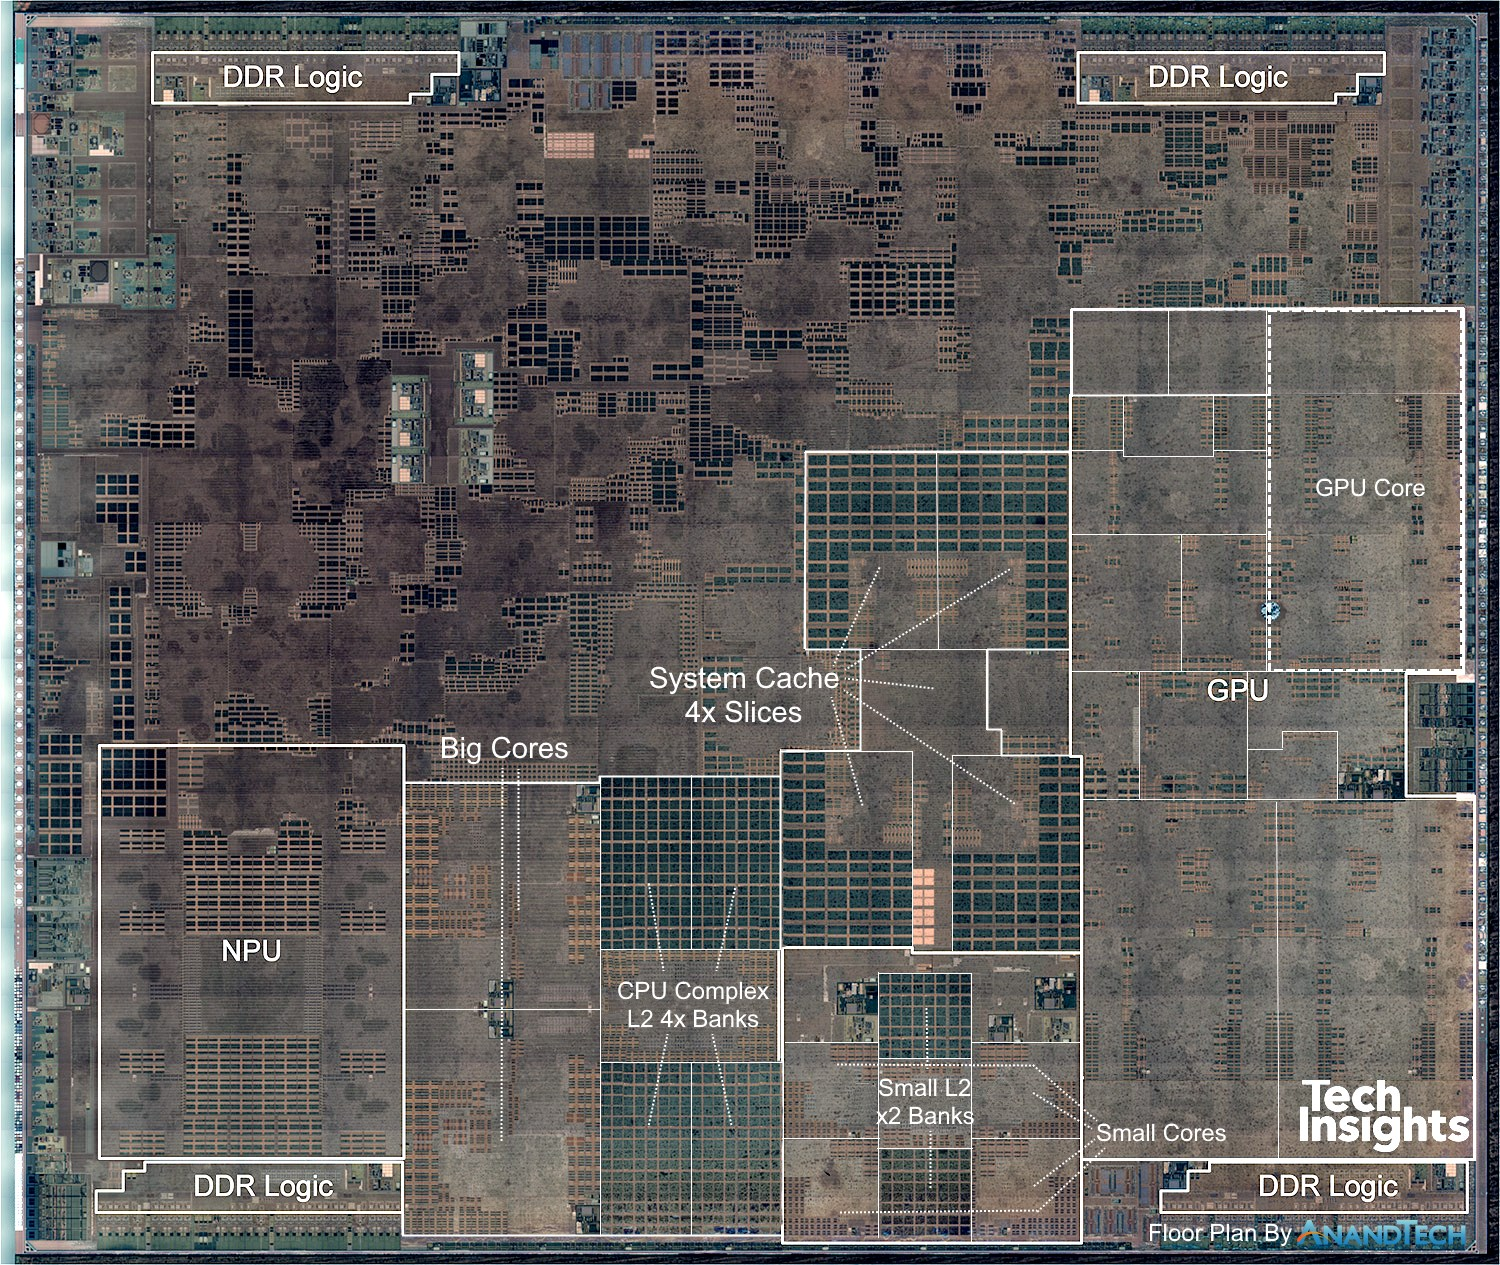
\includegraphics[width=0.8\linewidth]{images/AppleM1SOC.jpeg}
    \caption{ Apple M1 Architecture - (A12 Bionic) Chip floor plan~\cite{hollemans2020apple}}
    \label{fig:autoregressive_decoding}
\end{figure}

\subsubsection*{Unified Memory Architecture}
One of the defining features of the M1 SoC is its Unified Memory Architecture (UMA), which allows the CPU, GPU, and NPU to share the same memory pool \cite{hollemans2020apple}. This eliminates the need for memory copying across processing units and enables zero-copy execution. As a result, applications like retrieval-augmented generation (RAG) benefit from significantly reduced memory overhead and latency. Shared virtual addressing also simplifies software development by allowing seamless access to data structures across different compute units.

\subsubsection*{On-chip Accelerators: GPU and NPU}
The M1 chip includes a built-in GPU with 7--8 cores, capable of delivering up to 5.2 TOPS of performance in INT8 precision \cite{apple2020metal}. It supports general-purpose computation via Metal Shading Language (MSL), analogous to NVIDIA's CUDA, with added features like managed thread indexing and access to 7+ GB of RAM.

The Apple Neural Engine (ANE), or NPU, is an application-specific integrated circuit (ASIC) designed for efficient neural network operations. It offers 11 TOPS of INT8 compute and is exclusively used for machine learning tasks. However, it is only accessible via Apple’s CoreML framework, which supports Swift and Python interfaces. The NPU dynamically collaborates with the CPU, handling SIMD operations like matrix multiplication while delegating sequential logic to the CPU \cite{tinygrad2023apple}.

Unlike the GPU, the NPU is rarely used by general-purpose applications. This makes it a promising candidate for dedicated LLM inference workloads, as its usage is unlikely to interfere with the system's overall responsiveness.

\subsubsection*{Implications for Local LLM Inference}
The M1's integrated architecture is highly beneficial for deploying LLMs locally. Unified memory minimizes data movement, while the GPU and NPU offer parallel computation for matrix-heavy operations common in transformers. Although the NPU cannot be directly accessed via C++ (barring experimental reverse engineering efforts \cite{tinygrad2023apple}), its performance can be leveraged through CoreML model conversion pipelines \cite{apple2024coremlconvert}.

In the context of this project, these capabilities enable a lightweight, resource-efficient desktop application that performs real-time summarization and question answering over a user-provided corpus without relying on cloud resources.



% ============================================================
%
%                   CHAPTER 3: RELATED WORK
%
% =============================================================

\chapter{Related Work}
\label{ch:RelatedWork}
This chapter summarizes current research on Deep Learning (DL) that can be applied in Computational Fluid Dynamics (CFD) to support this study. It describes the current state of DL for CFD and discusses previous work done in this area that differs from this research. Additionally, it presents research that is outside of other areas that can be applied to CFDs.


%----------------------
\section{Potential areas of impact of DL in CFD}
\label{sec:DLinCFD}
%----------------------
The Computational Fluid Dynamics field deals with numerical simulations of fluid flows. Navier-Stokes equations are Partial Differential Equations (PDE) describing fluid flows. Solving those PDEs for chaotic (turbulent) flows requires computationally intensive numerical methods because of the necessary space and time scales. These turbulent flows can be simulated with different accuracy and resource costs. Data-driven modeling methods are revolutionizing scientific discoveries enabled by advances in scientific computing \cite{brunton_data-driven_2022}. Furthermore, Machine Learning and Deep Learning models have the potential to enhance those CFD simulations \cite{vinuesa_enhancing_2022} \cite{brunton_machine_2020}, and recently, there has been an emerging trend of research applications of ML and DL for CFD \cite{vinuesa_emerging_2022}. ML applications in CFD can be categorized into three main areas: Direct Numerical Simulation, Turbulent Modeling, and Reduce Order Models. 

\subsection*{\textbf{Direct Numerical Simulation}}
Direct Numerical Simulations (DNS) provide high accuracy for solving Navier-Stokes equations for fluid flows. Typically, there is a trade-off between the solution's accuracy and feasibility because solving this equation at scale is limited by the computational cost. Some proposed solutions focus on accelerating the numerical simulation by using Deep Learning to approximate parts of the computations involved. For example, \cite{kochkov_machine_2021} developed a method to accurately correct errors caused in low-resolution simulations by learning parameters affected by the coarse grid. They got stable results comparable to high-resolution numerical simulations and reduced the computational cost with a low-resolution discretization grid. Other research \cite{ajuria-illaramendi_towards_2020} \cite{ozbay_poisson_2021} focuses on using DL to solve the Poisson equation for corrections in incompressible fluids. This is done by exploiting data from previous examples to map deviations between uncorrected velocity and the resulting pressure field. 

Those methods only apply ML techniques in part of the solution but still rely on classical numerical methods to calculate the fluid flow. The solution proposed in this research is an end-to-end deep learning model that will apply DL to the entire simulation pipeline with a unified process. This simpler approach has the benefit of eliminating intermediate tasks in the simulation pipeline and thus reducing its complexity.

\subsection*{\textbf{Turbulent Modeling}}
Resolving direct numerical simulations is computationally expensive, so industry CFD applications use Reynolds-Averaged Navier-Stokes (RANS) and Large-Eddy Simulations (LES) methods. Various ML methods used to improve RANS turbulence modeling are explored in \cite{duraisamy_turbulence_2019} to improve its accuracy. Particularly the use of Physics-Informed Neural Networks (PINNs) \cite{wang_physics-guided_2023} \cite{eivazi_physics-informed_2022}. These PINNS models combine the data-driven modeling approach with using physics equations. This combined approach has the advantage of giving the model consistency with known physics laws; however, it makes the solution more complex to implement than a purely data-driven approach. 

In comparison, the model developed in this research is a data-driven approach that can learn from the given data to directly produce predictive results. This approach has the benefit of adapting to the particularities of each use case's data characteristics.


\subsection*{\textbf{Reduce Order Models}}
A useful application of ML in CFD is to develop Reduce Order Models (ROMs) to reduce the data complexity. This can be done because fluid flows contain principal structures that provide essential information about the flow. These ROMs represent the characteristics of the flow in a low-dimension representation that describes the evolution of those principal structures in the fluid, providing a substitute model for faster model predictions. A ROMs technique learns a low-dimensional coordinate system using Proper Orthogonal Decomposition (POD) \cite{taira_modal_2017} \cite{rowley_model_2017}. This technique is related to standard statistics and data-driven modeling techniques for dimensionality reduction: Principal Component Analysis (PCA) and Singular Value Decomposition (SVD) \cite{brunton_data-driven_2022}. Deep Learning can be used to perform those methods in dimensionality reduction by learning the subspace representation from the data \cite{lusch_deep_2018}. Autoencoders are neural networks where the input and output have the same dimensions, but in the middle, there is a bottleneck that reduces the dimensionality of the data. This type of model has two components: the first will take the input and compress it down to a smaller representation with fewer dimensions than the input, and the second one reconstruct the input from the representation. This low-dimensional representation subspace is called latent space and can simplify the original data by compressing it into a smaller representation. Autoencoders can be used to improve the performance of models that rely on classical ROM techniques. Because of the proven advantage of doing dimensionality reduction using DL Autoencoders, this model includes this type of component in its architecture.

%----------------------
\section{Related solutions of DL for CFD}
\label{sec:similarworks}
%----------------------
Recent works have validated the idea of using DL models for CFD modeling using different types of architectures and techniques. Here, we explore research examples that are the most relevant related work to this research, with similar goals but different solutions. It is important to note that although there are some similarities between them and this research, all of them have significant differences, mainly in the dataset used and the proposed architectures.

The use of an extended LSTM network with a Convolutional Neural Network (CNN) and Autoencoders was explored in \cite{mohan_compressed_2019} and \cite{han_new_2019}. Both used an Encoder-Decoder implemented with CNN to compress the data and an LSTM network enhanced with Convolutional filters that use the compressed data to generate the next part of the sequence. \cite{mohan_compressed_2019} develops a data-driven approach for Homogeneous Isotropic Turbulence data in a three-dimensional space. This solution is a sequence-to-sequence model, meaning it gets an initial sequence as input and produces the following sequence as output. The researchers proved that the model achieves good accuracy with long-term stability of the cyclic predictions while being very computationally efficient. \cite{han_new_2019} use a similar model with the same architecture for two-dimensional fluid flows around an obstacle. Their model shows similar results compared with flow fields calculated by a computational fluid dynamic solver. 

A similar method was proposed by \cite{hasegawa_cnn-lstm_2020} to develop ROMs for two-dimensional unsteady flows around a circular cylinder. They also used a CNN for the Autoencoder, with the goal of learning the temporal evolution of the flow in the latent space, they used a much simpler LSTM network. Additionally, they examined the accuracy dependence of this model with different Reynolds numbers (between 20 and 160). Their model was able to reconstruct flows with Reynolds numbers that were not used during the training of the model.

A DL approach to solving Partial Differential Equation systems was proposed in \cite{kakka_sequence_2022}. They developed a sequence-to-sequence model where the Autoencoder was implemented with a Convolutional LSTM. This model was tested with the moving MNIST dataset and the 2-D viscous Burgers equation. The researchers conclude that this model is an excellent network to use when predicting the time series of a dynamical system. Another solution for solving time-dependent PDEs was done in \cite{stevens_finitenet_2020} where they present a machine-learning approach based on a fully convolutional LSTM network to enhance finite-difference and finite-volume methods (FDM/FVM) common to solve PDEs. This method reduced the error by a factor of 2 or 3 compared to baseline algorithms.

A more advanced architecture of DL for CFD was recently proposed by \cite{wang_towards_2024}. The researchers explore the idea of using a combination of $\beta$-variational autoencoders ($\beta$-VAE) \cite{eivazi_towards_2022} to learn a compact representation of the flow velocity and transformers to predict the temporal-dynamics. They use a dataset of a flow around a square cylinder obtained using an open-source numerical simulation with a Reynolds number of 500. They also perform a study to find the optimal values for the $\beta$-VAE, and the effect on model’s performance of hyperparameters such as architecture complexity, regularization $\beta$, and latent vector size. Their model achieves excellent performance, with a 97.8\% of reconstruction accuracy and 96.5\% in temporal-dynamics predictions, demonstrating that this combination has the potential for developing ROMs in complex flows.


%----------------------
\section{Research from other domains}
\label{sec:ResearchOtherDomains}
%----------------------

We also explored other research ideas in the deep learning domain that are not related to CFD applications but can be extrapolated to be applied in this area. These ideas come from video analytics and weather forecasting. We explored how deep learning research in those areas can also be applied to CFD simulations.


\subsection*{\textbf{Video representation and prediction}}
The data for a fluid flow is a sequence of frames representing the state of the fluid at each time; in the same way, a video is a sequence of images in a timeline. Deep learning solutions that can learn features from videos for representation and future prediction have to deal with the same challenges as applications in CFD. In both cases, data has a spatio-temporal structure that requires the model to understand the space and time dimensions to predict future data. In \cite{srivastava_unsupervised_2015}, they use an LSTM neural network to learn representations of video sequences with an autoencoder and then extrapolate the learned video representations into the past and future. They also show that those representations help improve classification accuracy. The architecture is a composite model trained to perform two tasks simultaneously; using the encoded state, the model can predict the next frames as well as input reconstruction. They say that when done separately, the future predictor tends to only store information about the most recent frames, but when the model also has to reconstruct all of the input sequences, it cannot pay attention to just the last frames. This model performance was evaluated using the moving MNIST dataset and 300 hours of YouTube data. It was able to correctly predict the future frames, even when the objects superimpose or bounce while moving.


\subsection*{\textbf{ConvLSTM for precipitation nowcasting}}
Another area where analyzing spatiotemporal data to predict its future evolution is in weather. More specifically, the prediction of future rainfall intensity in a region over a short period of time, also known as precipitation nowcasting. In \cite{shi_convolutional_2015}, they propose a new type of neural network called ConvLSTM by extending the fully connected LSTM by adding convolutional structures. This end-to-end solution is able to outperform LSTM and state-of-the-art methods for the precipitation nowcasting problem. The main reason for this new neural network is that a fully connected LSTM has too much redundancy for spatial data. They mention that this network is not specific for precipitation nowcasting but can also be used for other prediction problems involving spatiotemporal sequence data.



% ============================================================
%
%                   CHAPTER 4: METHODS
%
% =============================================================

\chapter{Methods}
\label{ch:Methods}
This chapter covers the procedures involved in this research, from data collection to the proposed DL model's architecture and its training, how it is evaluated, and all the tools used during this study. It provides an explanation of how the solution for this study works and its justification.

%----------------------
\section{Data Collection}
\label{sec:DataCollection}
%----------------------
The dataset for this study consists of fluid flows interacting with an obstacle. Its purpose is to train and test the neural network solution proposed in this research. The fluid flows are generated using a numerical method, as is typically done in computational fluid dynamics simulations. The sequences represent the evolution of the fluid flow in space and time; therefore, this dataset could be considered two-dimensional Time Series data (See Section~\ref{sec:TimeSeries}).

Each fluid flow is a sequence of $400$ frames representing the state at a given time. The frames are a two-dimensional grid discretization of the simulated space, with a resolution of 200-width by 100-height cells. The values in the cells represent either the fluid's velocity at the position or -1 if it belongs to the obstacle. 

All the fluid flows in the dataset have a Reynolds number of 220 and flow from left to right, interacting with an obstacle with several dimensions and positions. These obstacles are either circumferences or ellipses, as shown in Figure~\ref{fig:cfd_obstacles}. Circumferences are simple shapes to model and are usually used to demonstrate fluid flow simulations. In contrast, ellipses are an easy simplification of an aircraft wing cross-section with different dimensions and inclinations (known as the ``angle of attack").

\begin{figure}[!h]
    \centering
    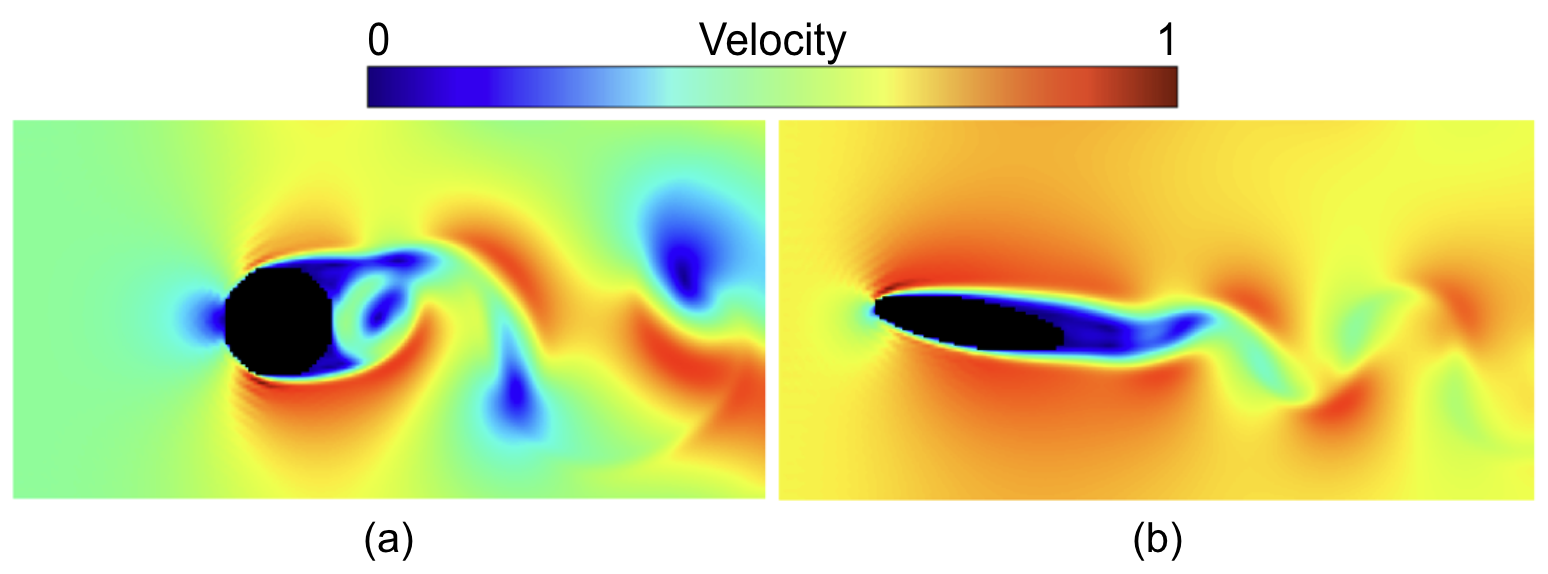
\includegraphics[width=0.9\linewidth]{images/cfd_obstacle_examples.png}
    \caption{Two CFD frames from different sequences showing the (a)circumference and the (b)ellipse obstacles}
    \label{fig:cfd_obstacles}
\end{figure}

In aeronautics, several pre-defined airfoils shapes (NACA airfoils) have been studied for the design of aircraft wings \cite{abbott_ira_h_summary_1945}; in particular, the NACA 2412 is used in the popular Cessna 172 Skyhawk. Figure~\ref{fig:naca_airfoils} shows examples of those airfoils. However, these shapes are very complex to calculate. As an alternative for this work, an ellipse shape was chosen as an approximation to the NACA airfoils. The ellipse geometry has a smooth, curved shape that can resemble the streamlined profile of the airfoil. It can provide a good approximation for the leading and trailing edges, capturing the essential aerodynamic characteristics while simplifying the complex geometry of the airfoil. This approximation is particularly useful for preliminary design and analysis, where exact precision is less critical. It allows for easier mathematical manipulation and analysis compared to the exact airfoil shape.

\begin{figure}[!ht]
    \centering
    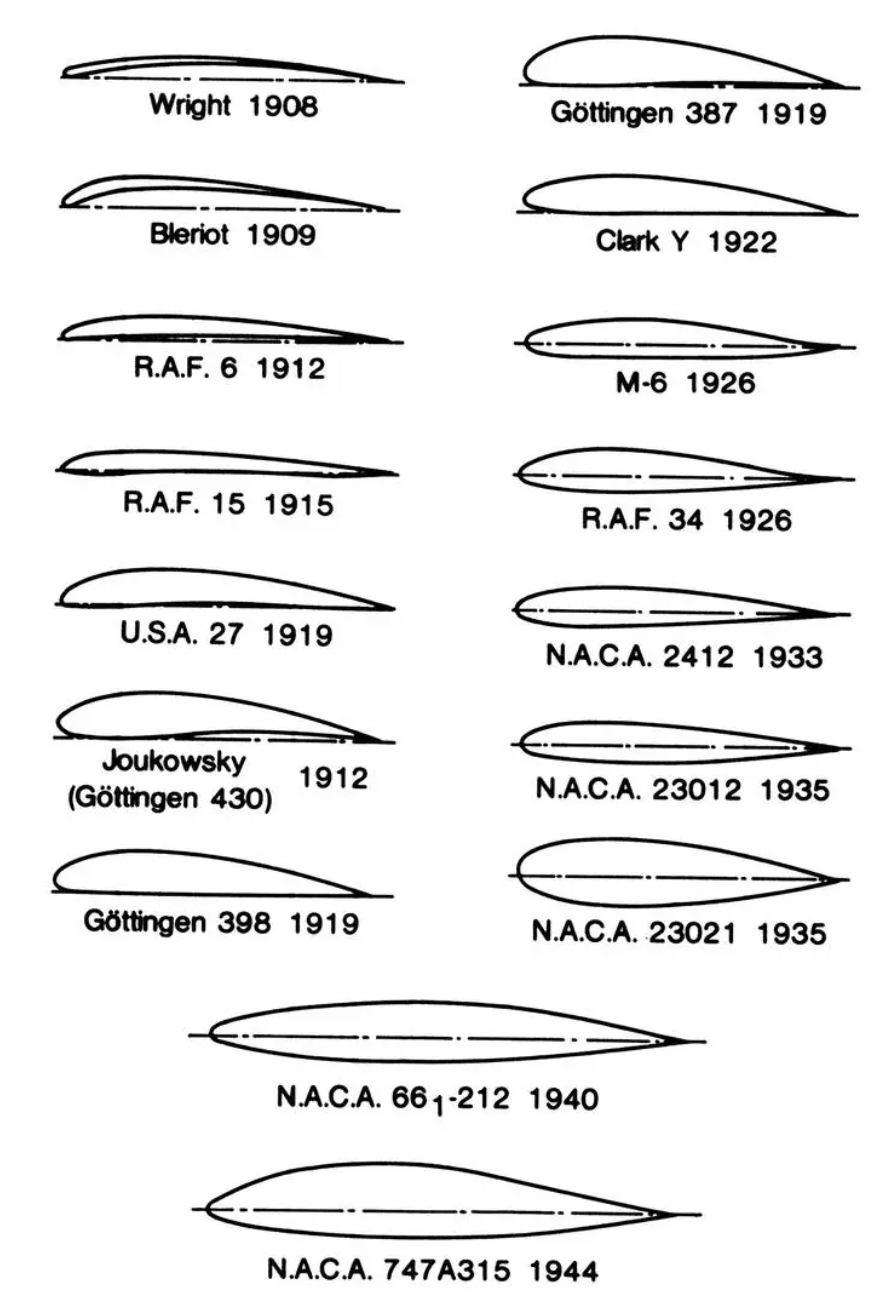
\includegraphics[width=0.6\linewidth]{images/naca_airfoils.png}
    \caption{The historical evolution of airfoil sections from 1908-1944. Credit: NACA-NASA}
    \label{fig:naca_airfoils}
\end{figure}

\subsection{Definitions}
The fluid flow sequence data can be represented in the following mathematical way. Data is taken from velocity observations in a spatial region on a $W \times H$ grid, which consists of $W$ columns and $H$ rows. Each grid cell has a velocity measurement that varies over time $T$.

\begin{defn}
    \label{defn:T}
    Let $T$ be a finite period of time and $t_i \in T$, where $i \in \{0,1,..., T\}$, is a time instance.
\end{defn}

We can then mathematically represent a fluid flow sequence as follows:

\begin{defn}
    \label{defn:fluid_flow_sequence}
    A fluid flow sequence is represented by a tensor $X \in \mathbb{R}^{T \times W \times H}$, where $x\in X$ and $x \in \mathbb{R}^{W \times H}$ is a velocity observation or fluid state at any given time $t \in T$.
\end{defn}

\begin{defn}
    \label{defn:window}
    Let $\mathcal{W}$ be a window of time $\subseteq T$, where $\mathcal{W}$ is of size $m$ and $1 < m < T$.
\end{defn}

When observations of $x \in X$ are recorded periodically over a time period $T$, we can think of them as a sequence of frames $x_0, x_1, x_2, ..., x_i, ..., x_T$. For this research, the spatiotemporal sequence generation problem is to generate the next most likely frame $x_i$ observation, given a window of previous observations $x_{i-m}, ..., x_{i-2}, x_{i-1}$. The problem can be formalized by equation~\ref{eq:generation-problem}, where $g$ represents the \textit{generate} function performed by the model.

\begin{equation}
    x_i = g(x_{i-m}, ..., x_{i-2}, x_{i-1}) 
    \label{eq:generation-problem}
\end{equation}

% -------------------------------------------------------
\section{Data Preparation}
\label{sec:DataPreparation}
% %-------------------------------------------------------
Before the data is used to train and evaluate the model, the following preprocessing steps are applied to transform the data: 1) data normalization, 2) data slicing, and 3) dividing the dataset into a training and testing set.

\begin{enumerate}
    \item \textbf{Data normalization:} First, the data is normalized by scaling the velocity values between 0 and 1. This data normalization improves the gradient descent optimization during the neural network's training, which is a common requirement for deep learning methods. This scaling is done according to Equation~\ref{eq:min-maxscaling} below.

        \begin{equation}
            v_{scaled} = \frac{v-v_{min}}{v_{max} - v_{min}}
            \label{eq:min-maxscaling}
        \end{equation}
    
    This scaling technique provides robustness to very small standard deviations in the dataset's velocity values. During this process, the obstacle cells are left with a value of -1 to distinguish them from the fluid while maintaining the velocity values in the 0 to 1 range.
    
    \item \textbf{Data slicing:} This step focuses on creating simulated sub-sequences to train the model. The input and output datasets are generated using the original dataset, which consists of the simulated [fluid] sequences. The model takes as input a specific window $\mathcal{W}$ consisting of $m$ frames from the simulated sequence of size $T$; it then uses this window to generate the next frame. Since $m<T$, the length of the input dataset elements must be reduced to match the this window. To do this, each original sequence is segmented into sub-sequences of length $m$ (size of $\mathcal{W}$). After segmenting the original sequence of size $T$, it results in more than one sub-sequence of size $m$ in the input dataset.
    
    Figure~\ref{fig:data_slicing} illustrates this process, where the input dataset to the model (the set of fluid sub-sequences $X$ of size $m$ over a time window $\mathcal{W}$ using definition~\ref{defn:window}), will be used to generate the output set (the next set of frames). During the training step, the model will learn how to infer $x_t$ from the previous $m$ frames (see  Equation~\ref{eq:generation-problem}).
 
    \begin{figure}[H]
        \centering
        % 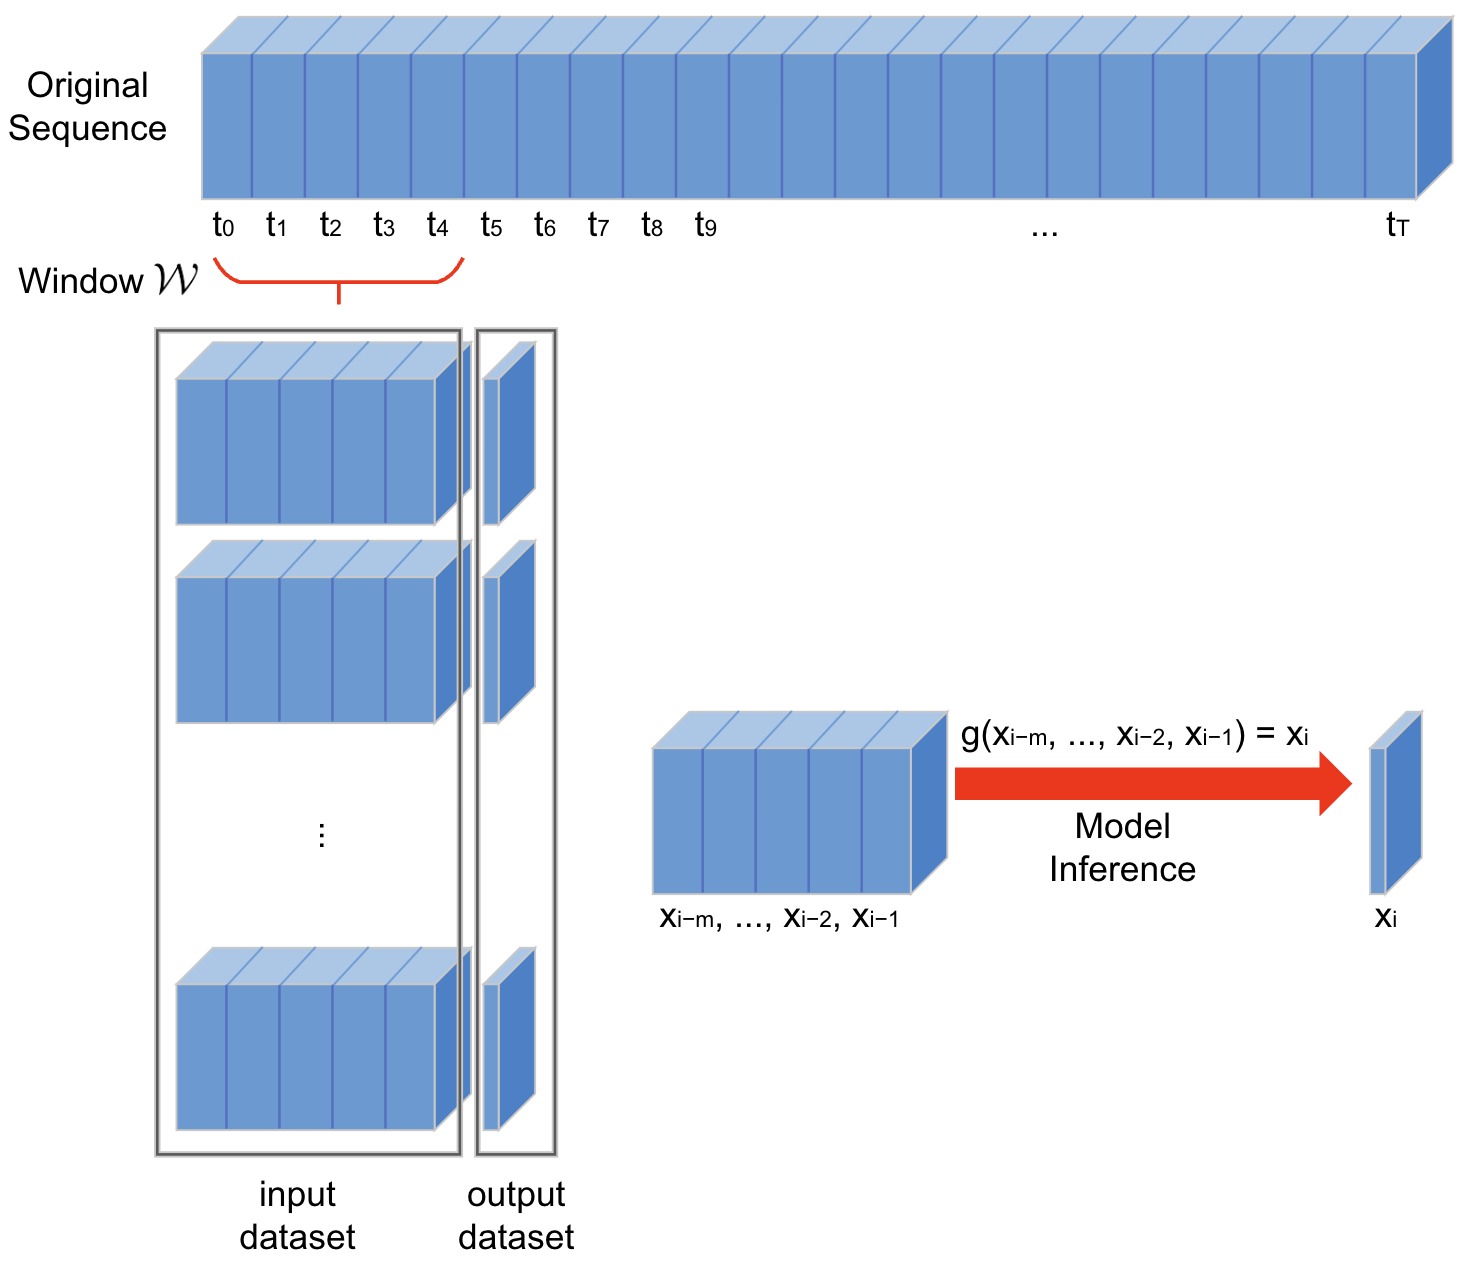
\includegraphics[width=0.9\linewidth]{images/data_slicing.png}
        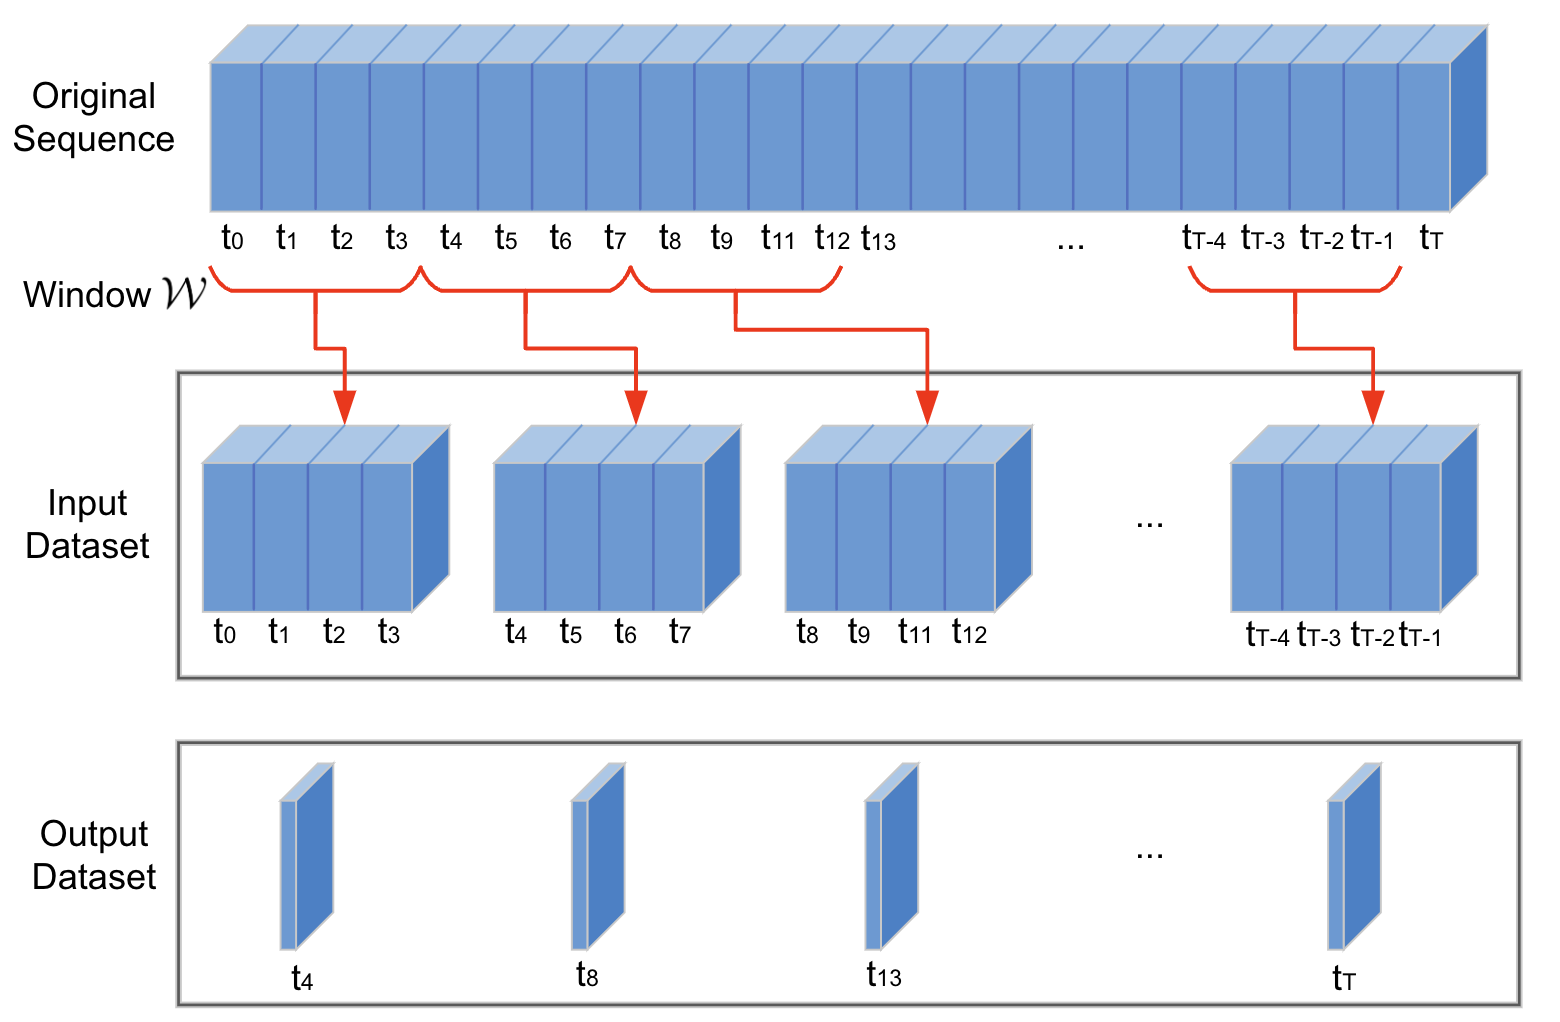
\includegraphics[width=0.9\linewidth]{images/data_slicing_v2.png}
        \caption{Slicing of sequence into $\mathcal{W}$ sub-sequences used to train the model.}
        \label{fig:data_slicing}
    \end{figure}

    \item \textbf{Training, Validation, and Testing sets:} Finally, the dataset is shuffled and then randomly divided into training, validation, and testing sets with an 8:1:1 ratio, respectively. This is done to validate and test the model using the cross-validation method with samples not used during training. This aims to provide an unbiased evaluation of the model's efficacy, which -- ideally --  should appropriately generalize (for new data) without over-fitting (training data). 
    
\end{enumerate}


%----------------------
\section{Model Architecture}
\label{sec:ModelArchitecture}
%----------------------
The DL solution proposed in this research is an end-to-end model, meaning it will perform all the tasks from data input to generating the fluid flow simulation output in one unified process. In contrast, other related research uses machine-learning or DL techniques for only a specific part of the simulation, leaving the rest to a classical numerical method and making the process more complex. A benefit of our simple approach with only one task is eliminating the need for complex pipelines between separate parts in the simulation process, thus reducing development time and potential sources of error. Additionally, end-to-end models can better adapt to diverse datasets and changing environments since they learn directly from raw data, capturing intricate patterns and relationships that might be missed in traditional approaches, like DNS.

The goal of this model is to generate predictions of a fluid flow's evolution. To accomplish this, the model looks at past states in the flow and generates the following future state. The future state can then be used as an input to continue generating new states in the simulation. This step can be repeated as many times as necessary as a feedback loop shown in Figure~\ref{fig:feedback_loop} below. As a result of this feedback loop, the model can produce a long fluid flow sequence. In Figure~\ref{fig:feedback_loop}.a we can see how the resulting frame is put at the end of the input sequence to generate a new frame (see Section~\ref{subsec:Generator}). Figure~\ref{fig:feedback_loop}.b shows how the model looks at a certain window of the frame and moves forward in time to generate the rest of the sequence. At the beginning of a simulation, the model uses an initial condition or ``ground truth" represented by a number of frames equal to the sliding window ($\mathcal{W}$). As $\mathcal{W}$ slides, new frames are generated, which are in turn used to generate more subsequent frames. Eventually, an entire sequence can be generated, knowing only the first frames from the initial fluid's condition, and the rest are completely generated by the model.

\begin{figure}[!htbp]
    \centering
    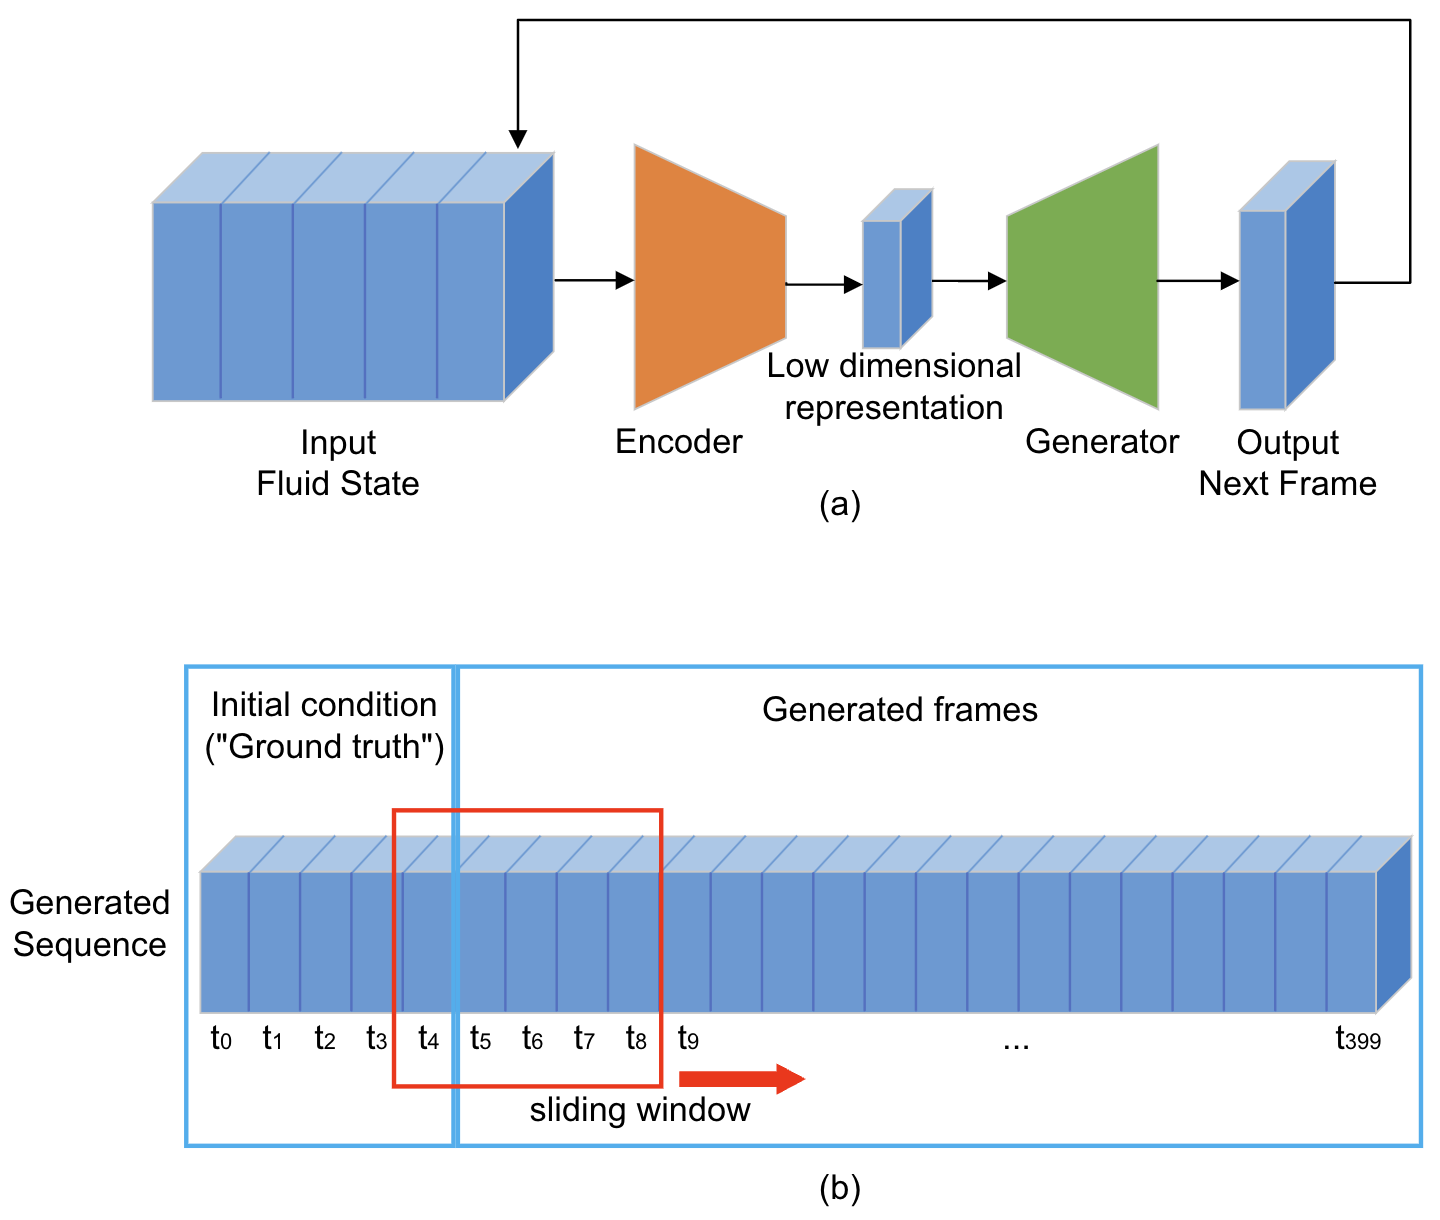
\includegraphics[width=1\linewidth]{images/feedback_loop.png}
    \caption{Diagram showing a) the flow between the model's main components and b) sliding window approach for prediction.}
    \label{fig:feedback_loop}
\end{figure}

Because of the data's spatiotemporal characteristics, the neural network has to be capable of analyzing and learning the evolution of fluid flows in two dimensions: space and time. A CNN (See Section~\ref{sec:CNN}) can help understand the spatial structure of the fluid to extract the flow's features and patterns in space. Additionally, the model needs to ``remember" what happened in the past to produce the next state, so it needs a memory mechanism that can be provided by a recurrent neural network such as an LSTM (See Section~\ref{sec:LSTM}), commonly used in Natural Language Processing tasks. As mentioned before, these two types of neural networks have been combined to create the ConvLSTM (See Section~\ref{sec:ConvLSTM}) as an extension of the LSTM network that can also ``look" for features in space and time. For this reason, the ConvLSTM network was chosen to implement the neural network architecture proposed in this study.

Because this data has many dimensions and complexities, a dimensionality reduction is applied to capture the principal components of the flow before generating the next frame. This ensures that the model will rely on a minimal representation of the fluid flow that accurately describes its behavior. For this model architecture, the dimensionality reduction is implemented by an Autoencoder (See Section~\ref{sec:Autoencoders}) neural network that can produce it as part of the same model.

\begin{figure}[!htbp]
    \centering
    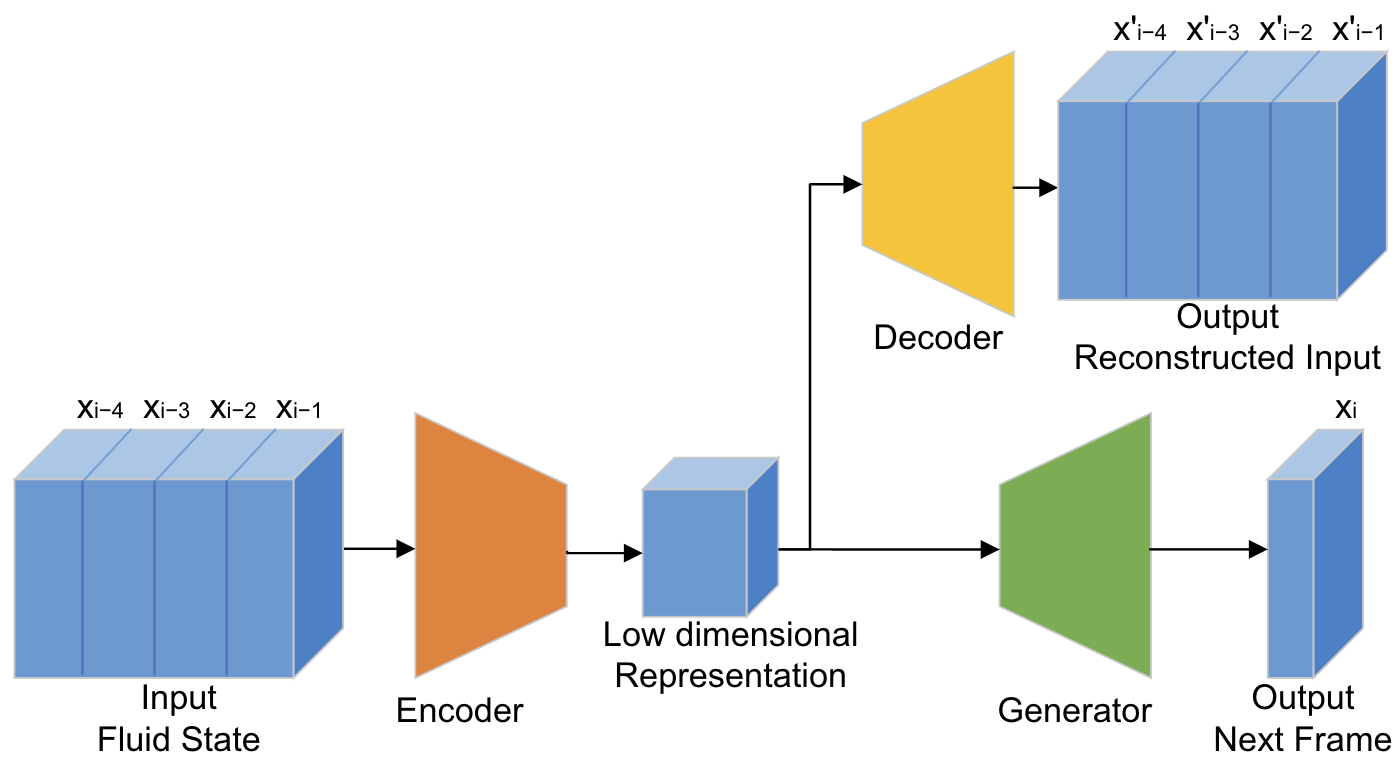
\includegraphics[width=0.8\linewidth]{images/model_schematic.png}
    \caption{Schematic diagram of the model architecture}
    \label{fig:model_schematic}
\end{figure}

In summary, the model has two main parts, as shown in Figure~\ref{fig:model_schematic}: 1) an Encoder that reduces the data's dimensionality and 2) a Generator that gets a representation of the past frames and creates the next one.

\subsection{Encoder}
\label{subsec:Encoder}
The Autoencoder is a neural network architecture composed of an Encoder and a Decoder, and it is used for dimensionality reduction (See section~\ref{sec:Autoencoders}). It takes data with many dimensions and creates a representation of this data in a lower-dimensional space. It is used similarly to classical statistical methods, such as singular value decomposition or principal component analysis. As explained in the related works chapter~\ref{ch:RelatedWork}, autoencoders were previously used for fluid flow analysis, such as identifying the main components in a fluid flow and identifying eddies in the flows. It has also been used for dimensionality reduction for other methods that are not deep learning models. 


\subsection{Generator}
\label{subsec:Generator}
The generator takes the lower-dimensional representation of the fluid flow state and generates a new frame in the sequence. Using a lower representation of the data instead of all the original dimensions makes this work easier because the generator will get as input the main components that can describe the flow. 


%----------------------
\section{Model training}
\label{sec:ModelTraining}
%----------------------
The Encoder is trained in conjunction with the Decoder component, which takes the lower dimensionality representation and tries to reconstruct the original input. If the decoder can reconstruct the original data using the reduced representation from the encoder, this means that the representation captures the main elements of the sequence, and the encoder works correctly. This decoder is auxiliary and discarded once the model’s training is completed.

Cross-validation \cite{bengio_practical_2012} is used to ensure that the model performance generalizes well to unseen data during training. This method, commonly used in machine learning, involves splitting the dataset into three parts: a training set, a validation set, and a testing set. The training set is used to train the model, and simultaneously, the validation set is used to evaluate the model's performance during training. Once the model is trained and optimized, it is tested on a separate and unseen test dataset to assess its generalization performance. This technique also helps prevent overfitting by providing an independent dataset for model evaluation. It ensures that the model's performance estimates are more reliable and indicate its performance on new data.

The neural network training job was distributed across the two GPUs available on the server. This was done using the Mirrored Strategy, a synchronous data parallelism algorithm for neural network training. This algorithm replicates the model on both GPUs and splits the dataset between devices. The CPU prepares and sends the data batches to the GPUs. During training, each GPU performs a forward pass over the model on different input data to compute the loss function; subsequently, gradients are calculated on each device based on that loss. Both sets of gradients are then combined with an all-reduce operation by averaging them and re-distributing them across devices to update the model parameters on each replica, synchronizing them. This process is repeated for each data batch for every training epoch.


%----------------------
\section{Hyperparameter Optimization}
\label{sec:HyperparameterOptimization}
%----------------------
The model architecture and training have specific characteristics or hyperparameters that can take various possible values. These hyperparameters impact the model's performance, i.e., different combinations of such values may result in different model efficacy; consequently, it is important to find a suitable hyperparameter combination to optimize the model efficacy.

Hyperparameter optimization with Random Grid Search \cite{bengio_practical_2012} in ML involves systematically exploring a predefined hyperparameter space by randomly sampling combinations of hyperparameters, rather than exhaustively searching through all possible such combinations. This approach helps efficiently find an optimal set of hyperparameters for the model by balancing computational resources and exploring the parameter space. Random grid search randomly selects hyperparameter values from specified distributions and evaluates each combination using cross-validation to determine the set that yields the best performance metric. This technique can effectively search a large hyperparameter space, improving model performance without exhaustive computational costs.

The hyperparameters considered for this model are:

\begin{itemize}
    \item Learning rate: it determines the update step size of the weight in the neural network at each iteration during the optimization process, i.e., the loss function moving towards a minimum. A high learning rate can lead to rapid convergence at the risk of overshooting the optimal solution, causing the model to diverge. On the other hand, a low learning rate ensures steady convergence at the sake of a slower training process which can get stuck in local minima. This parameter significantly impacts the efficiency and effectiveness of the model training. The best training results were achieved with a learning rate of 0.001.
    
    \item Number of layers: the number of neural network layers affects the \textit{capacity} of the model to learn complex representations. In the context of this research, more layers can enable the model to capture more hierarchical features and intricate patterns in the fluid-flows. This can improve the model's performance. However, having more layers makes the model more complex and more susceptible to overfitting the training data. The model achieved the best results using 3 ConvLSTM layers on each Encoder and Decoder component and 4 ConvLSTM layers in the Generator component.
    
    \item Number of filters or kernels on each layer: convolutional filters detect spatial features in the input data. These filters enable the model to capture both spatial and temporal dependencies in the fluid flow. The number of filters impacts the model's ability to extract relevant features. Having more filters can capture more complex data patterns but at the cost of increasing computational cost. This parameter affects the accuracy and efficiency of the model. In the ConvLSTM layers of the Autoencoder, this model architecture got the best results using 64 filters in the first and last layers and 32 in the other ones. In the Generator component, the first layer uses 32 filters and 64 in the rest.
    
    \item Size of the filter: this refers to the convolutional filters' dimension to capture features of the input data. The filter size determines the scope of the local spatial region examined by the model. Larger filters can capture broader spatial patterns but may miss fine-grained details, while smaller filters focus on more localized features, potentially overlooking broader context. This impacts the model's ability to detect relevant features. The following filter sizes in the ConvLSTM layers of the architecture were used to get the best results, in order from the first to last layer of each component: the Encoder has filter sizes of 4 by 4, 3 by 3, and 2 by 2; the Decoder has filters of 2 by 2, 3 by 3, and 4 by 4; and the Generator filter sizes are 3 by 3 for all of its layers. 
\end{itemize}

In order to define a search space of hyperparameter combinations, a range of values is set for each of these hyperparameters.  Potential combinations are selected by random sampling, then a model is trained using those combinations, and the one with the best performance is selected. Once the best combination is found, the model is trained during more epochs to get the final version of the model.

When choosing the $m$ size of the window $\mathcal{W}$, several aspects were considered, e.g., the amount of ``historical'' data used to generate a prediction. Similar to the Exponential Moving Average (EMA) heuristic \cite{kalekar_time_2004} \cite{ugli_cognitive_2023}, which can be used in time-series forecasting scenarios and LSTM models to weight the amount and relevance of historic measurements vs. predicted ones. In our case, we can think of $m$ as the amount of historical information that the model will receive to make a future prediction. In this sense, using a small window will not give enough information to the model. On the other hand, having a bigger window size provides more information and is better for the model, but if $m$ is too big, it will need too much historical information, making the model pointless. Additionally, a bigger window expands the input dimensions, so more computations would be required to compress the data to create the lower dimensional representation. This increase in computations makes the model slower to execute and train, which given our limited computational resources, could render our model impractical. In addition, since the sequences have 400 frames each, the window size $m$ has to be a divisor of 400 to split them into sub-sequences for data preparation, as explained in \ref{sec:DataPreparation}. Overall, since a window of size 2 would be too small to provide the model with enough information, a window size of 4 was chosen since it is the smallest $m$ that allows for the even division of sub-sequences while keeping the model practical.


%----------------------
\section{Proposed Architecture Details}
\label{sec:ArchitectureDetails}
%----------------------

The final model architecture has two components: the \textbf{Autoencoder} and the \textbf{Generator}. The Autoencoder is divided into the Encoder and Decoder. The window $\mathcal{W}$ of $m=4$ frames is first input into the Decoder, which creates a low-resolution representation of the simulation. Next, this low-resolution representation is input into the Generator to create the next frame state of the fluid flow. All these components are implemented in the neural network by a set of ConvLSTM layers followed by either MaxPooling or UpSampling layers. ConvLSTM layers extract features in the data by using convolutional operators called filters or kernels. MaxPooling and UpSampling layers compress or uncompress the intermediate data outputs between ConvLSTM layers. MaxPooling downsamples the input by taking the maximum value in the kernel window along the spatial dimension. UpSampling layers resize the input by interpolating its values. Figure~\ref{fig:model_detail} shows a detailed diagram of this architecture where we can see the order of these layers. In the Encoder, successive layers of ConvLSTM and MaxPooling layers downsample the data, resulting in a representation that is half the input size. This representation is then reconstructed in the Decoder by upsampling it using UpSampling and ConvLSTM layers. Each of these layers has a different amount of filters or pool windows of different sizes, respectively. 
Figure~\ref{fig:model_detail} also shows the output dimension of each layer.

\begin{figure}[!htbp]
    \centering
    \makebox[\textwidth][c]{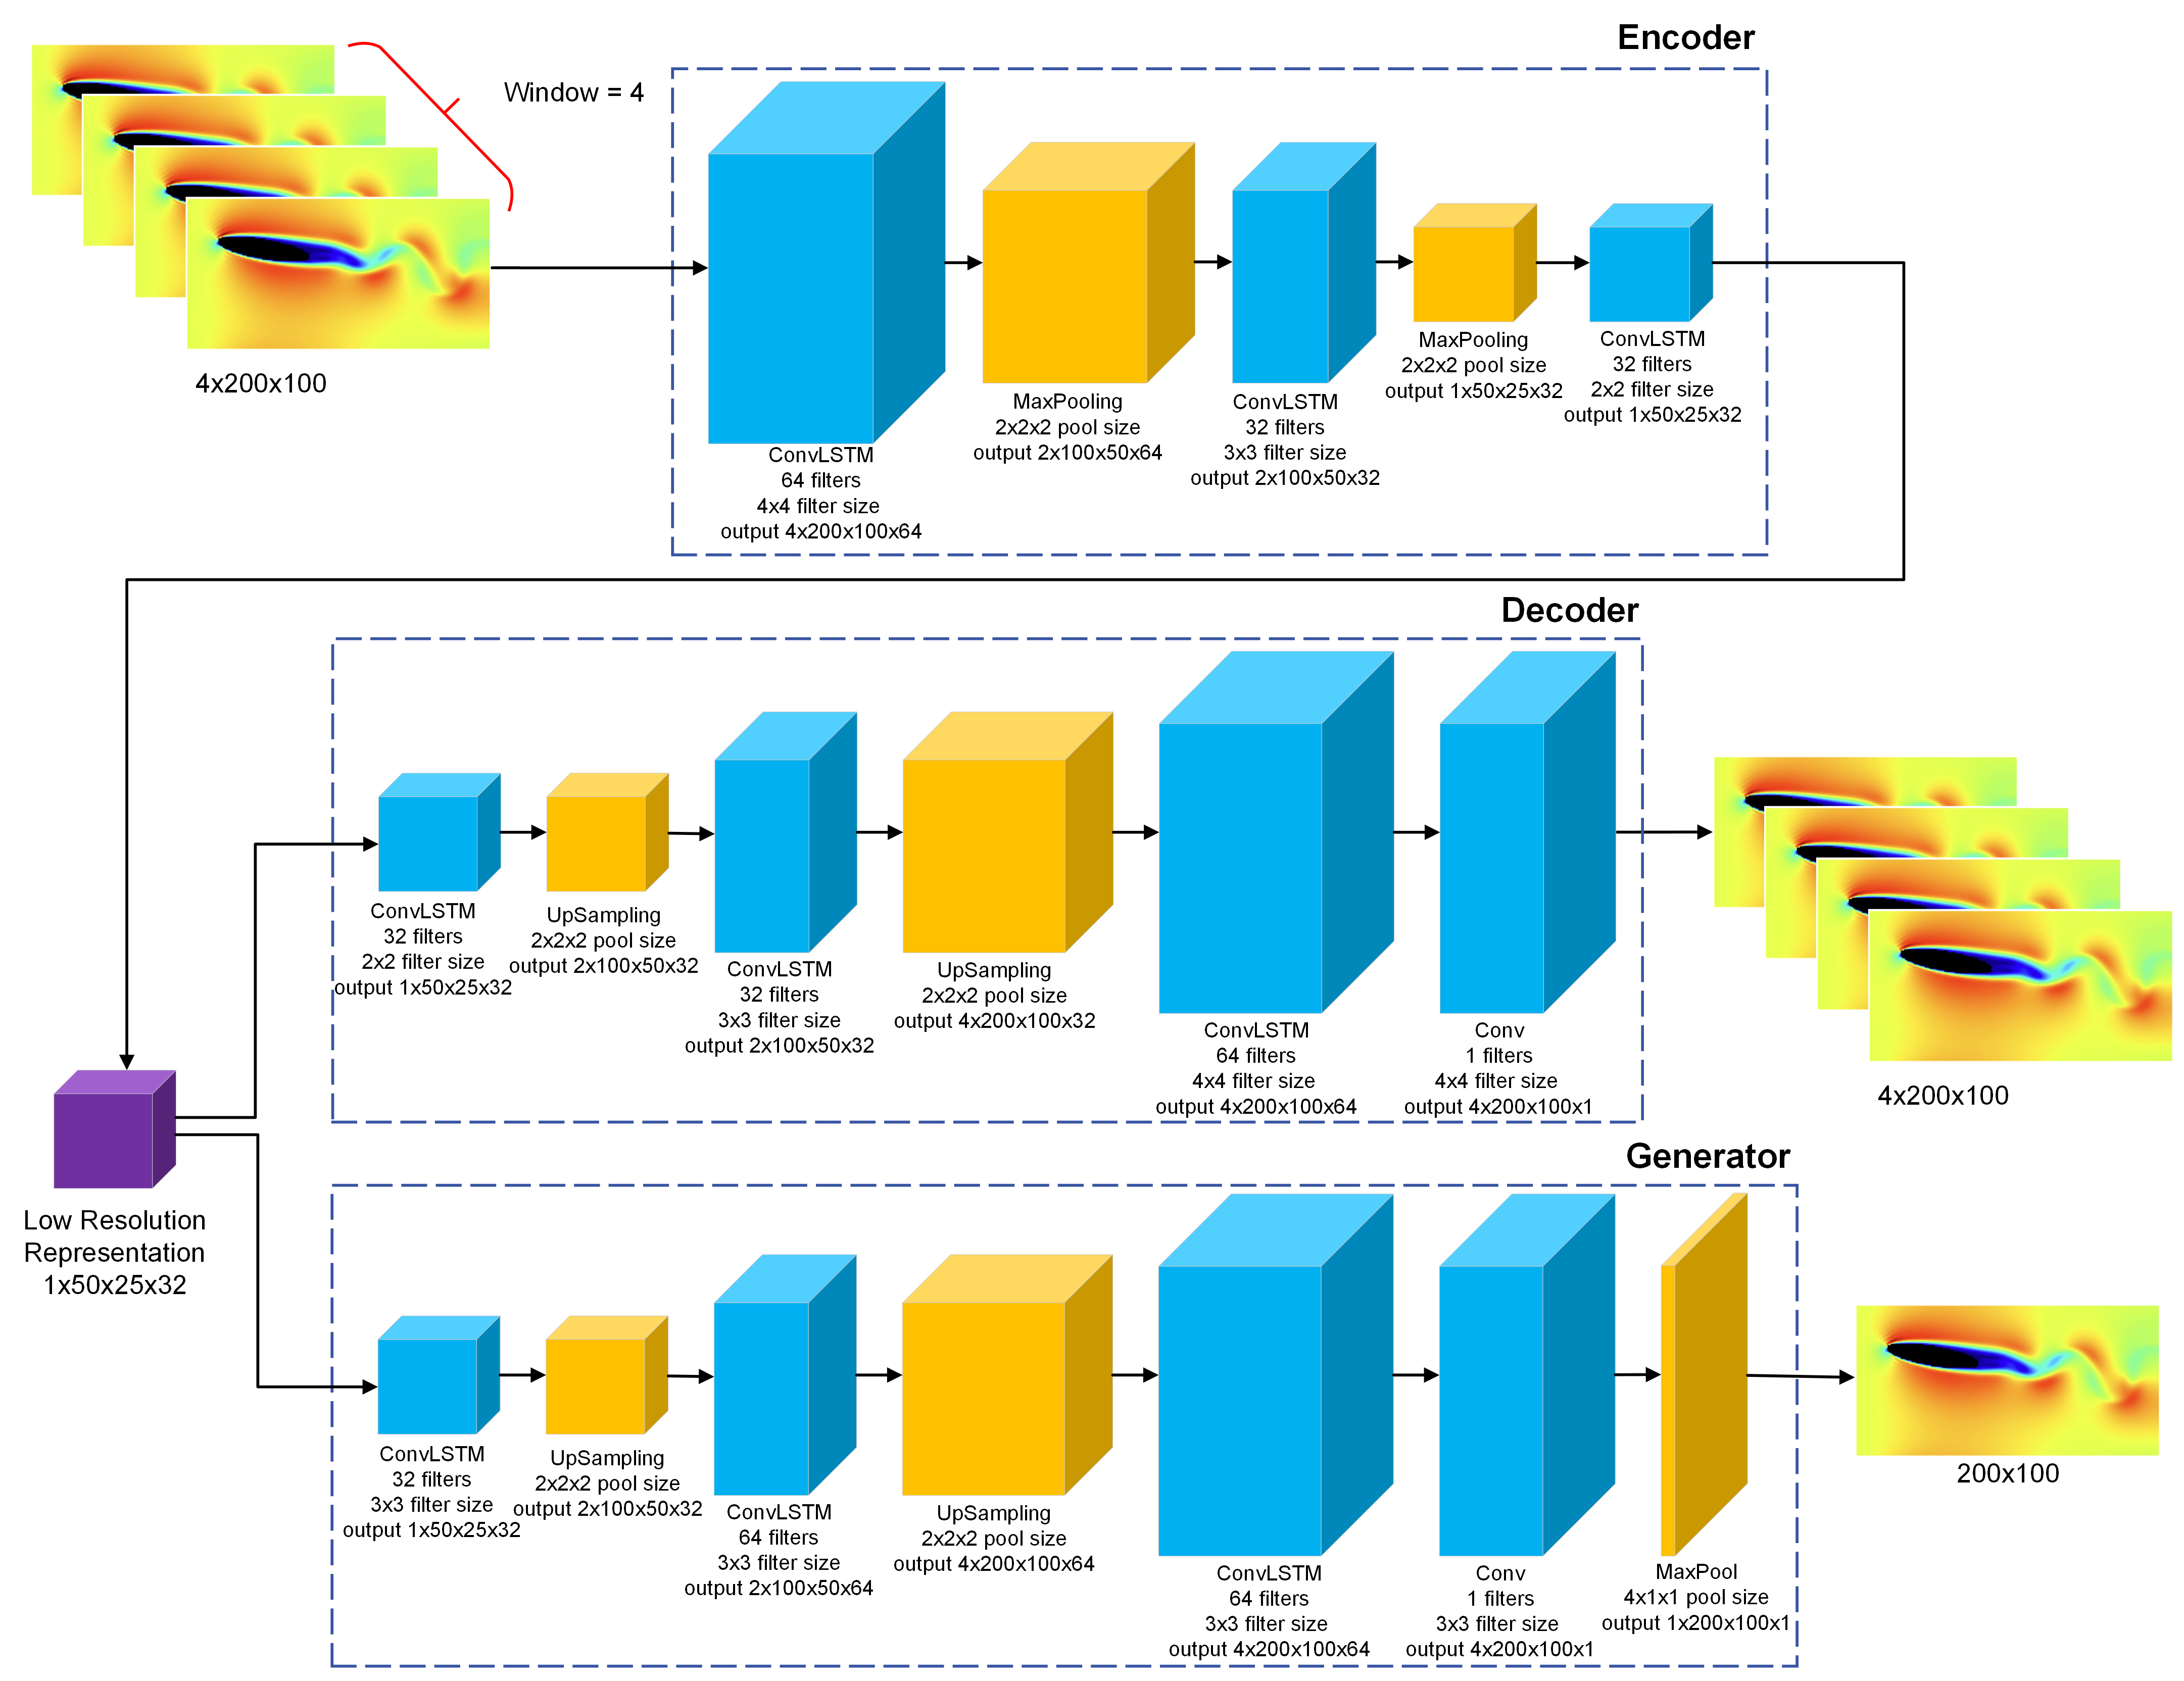
\includegraphics[width=1.3\textwidth]{images/architecture_detail.png}}
    % 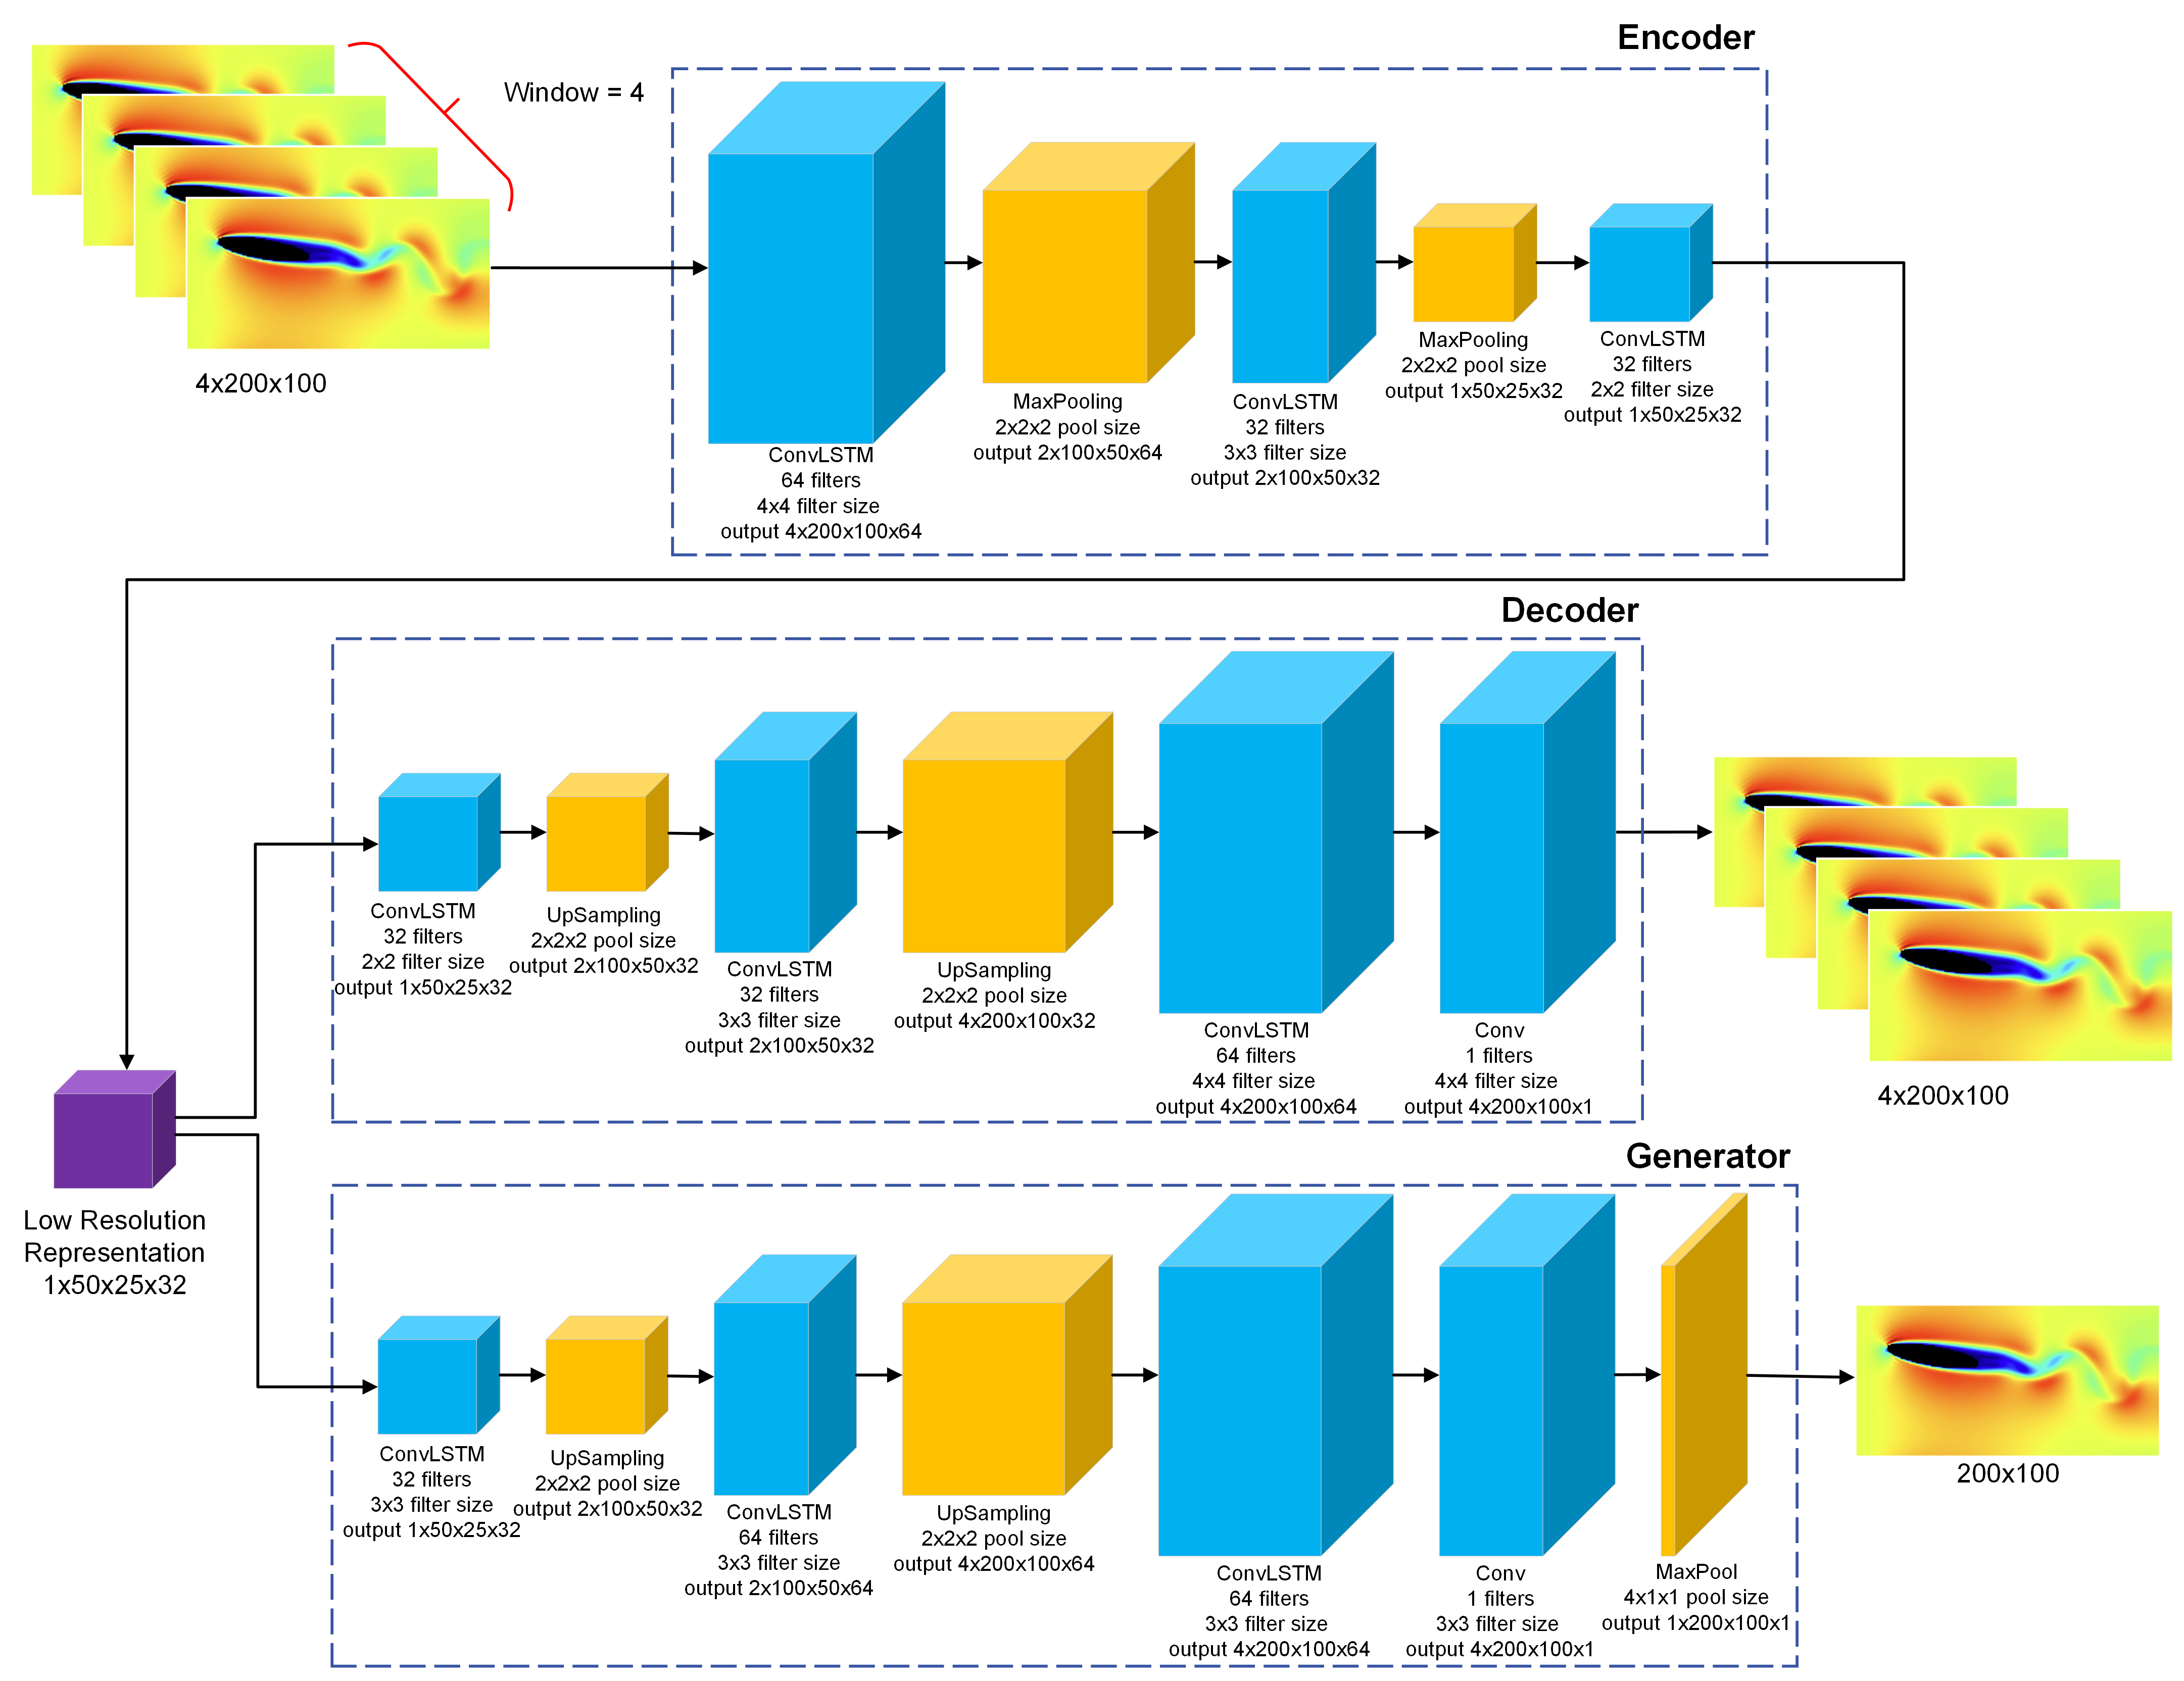
\includegraphics[width=1\linewidth]{images/architecture_detail.png}
    \caption{Detail diagram of the model architecture}
    \label{fig:model_detail}
\end{figure}

%----------------------
\section{Evaluation Methods}
\label{sec:EvaluationMethods}
%----------------------
The model evaluation is done using three strategies:
\begin{enumerate}
    \item Calculating the Mean Square Error between the original and generated simulations.
    \item Visually inspecting the simulation result by rendering an image with the generated data and comparing it with the expected data (the ground truth).
    \item Creating a histogram of frame values for the original and the generated data, these will be compared ``side-by-side" to analyze similarities and identify possible drastic differences.
\end{enumerate}

%----------------------
\section{Software and Tools}
\label{sec:SoftwareandTools}
%----------------------
For the implementation of all the methods described in the previous section, the Python \cite{python} scripting language with the following libraries: TensorFlow \cite{tensorflow} and Keras \cite{keras}, for the neural network implementations and training; Numpy \cite{numpy} and scikit-learn \cite{scikit-learn}, for data manipulation and preprocessing; and Matplotlib \cite{matplotlib}, to generate the plots and visualizations.

VS Code was used as an IDE for code implementation, and data analysis of the results was done using Jupyter Notebook \cite{jupyter}.

The server used for training and evaluation of the neural network model has the hardware specifications described in Table \ref{tab:serverHW} below.

\begin{table}[h]
    \caption{Server Hardware specifications}
    \centering
    \begin{tabular}{|c|l|}
    \hline
    \multirow{3}{*}{CPU} & Intel(R) Xeon(R) Gold 5118 CPU       \\
                         & 2.30GHz of frequency                 \\
                         & 12 cores                             \\ \hline
    RAM                  & 192 GB                               \\ \hline
    \multirow{3}{*}{GPU} & 2x Nvidia Tesla V100 with 16 GB or RAM each \\
                         & Nvidia Volta Microarchitecture       \\
                         & Compute Capability 7.0               \\ \hline
    \end{tabular}
    \label{tab:serverHW}
\end{table}



% ============================================================
%
%                   CHAPTER 5: RESULTS
%
% =============================================================

\chapter{Results}
\label{ch:Results}

This chapter covers the experiment design and setup, describing in detail results obtained during different phases and tests. This chapter is organized as follows: first, we discuss the results of the training and its validation in Section~\ref{sec:TrainingResults}, then in Section~\ref{sec:AutoencoderResults} and Section~\ref{sec:GeneratorResults} we explore the DL model performance from the perspective of each component individually using the methods defined in Section~\ref{sec:EvaluationMethods}.  Lastly, in Section~\ref{sec:ModelPerformance}, we analyze the performance of the DL model based on the two main evaluation metrics defined in Section~\ref{sec:ResearchObjectiveandSolution} (MSE and execution time).

Results from experiments in this chapter are based on the dataset described in Section~\ref{sec:DataCollection}. The experiments performed can be categorized into two main types based on the obstacle shape used:
\begin{enumerate}
    \item Circular obstacle: the obstacle is randomly positioned in the simulation space, and its size is given by radius $\textbf{r} = qH$, where $q \in [\frac{1}{9}, \frac{1}{5}]$ and $H$ is the height of the simulated region.
    
    \item Elliptical obstacle: the obstacle is also randomly positioned in the space, and its size is given by semi-major axis $\textbf{a}=qH$, where $q \in [\frac{1}{5}$, $\frac{1}{3}]$ and $H$ is the simulated region height, and the semi-minor axis $\textbf{b}=p\textbf{a}$, where $p \in [\frac{1}{5}, \frac{1}{4}]$. The ellipse is also tilted with an angle $\boldsymbol{\alpha} \in [-30^\circ, 30^\circ]$ with respect to $\textbf{a}$ and the Cartesian $x$-axis.
\end{enumerate}

The ranges of the obstacle dimensions and positions were chosen to fully fit the shape inside the simulated space without touching its perimeter. The dimensions of the Ellipse object were chosen to maintain a shape similar to that of an airfoil as described in Section~\ref{sec:DataCollection}, and its inclination range to represent common wing ``angle of attack" including the critical or stalling ``angle of attack" (typically between $18^\circ$ and $25^\circ$ degrees)\cite{abbott_ira_h_summary_1945}.


%----------------------
\section{Training Results}
\label{sec:TrainingResults}
%----------------------

The neural network was trained for 500 epochs, across which, the Mean Squared Error (MSE) loss functions results were collected for both the Autoencoder and the Generator. The training error is captured in  Both plots in Figure~\ref{fig:loss} show that the is generally lower than the validation error; this is to be expected given the proposed model was evaluated with sequences used during the training process. 

\begin{figure}[H]
    \centering
    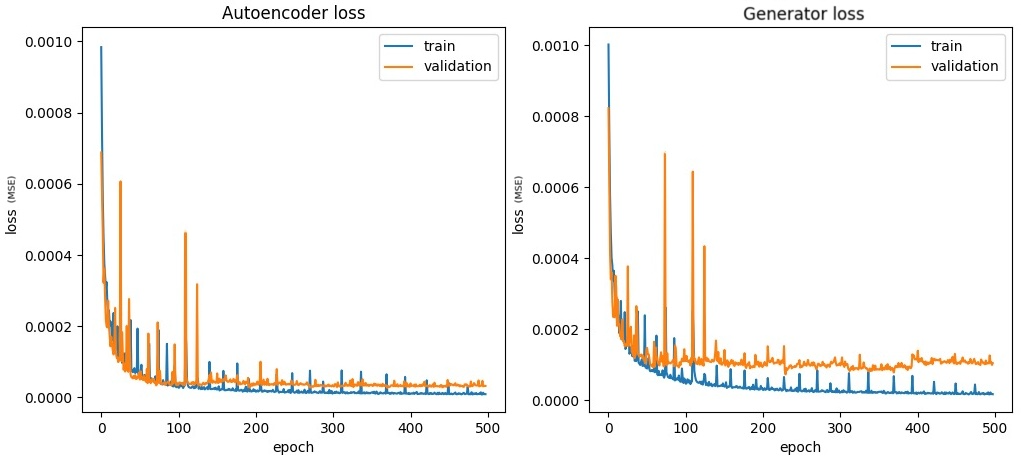
\includegraphics[width=1\linewidth]{images/model_training.png}
    \caption{Autoencoder and Generator loss evolution during training}
    \label{fig:loss}
\end{figure}

Figure \ref{fig:loss} demonstrates the stability of the MSE loss function's evolution during training. The loss trend quickly descends, and after 200 epochs, the error stabilizes and converges to its final value. In addition, note that the slight difference between the training and validation errors signifies that the model does not excessively over-fit the training data. Regular error spikes appear during training, representing instances where the model encountered local maximums before finding a local minimum. This happens when, during parameter optimization, a new combination of the network’s weights is worse than the previous one, but then it improves again. This further underscores the model's reliability. These spikes decrease as the training advances, indicating a stable and reliable training process. Another critical aspect to note is that those spikes happen almost on the same epoch number and with a similar intensity for both of the model's components (Autoencoder and Generator), meaning that these components are working in collaboration to find the best result. This supports the election of the model architecture.

\begin{table}[h]
    \caption{Training and Testing errors (MSE)}
    \centering
    \begin{tabular}{|c|c|c|}
    \hline
             & Autoencoder & Generator \\ \hline
    Training & $7.7727\times10^{-06}$ & $1.5429\times10^{-05}$ \\ \hline
    Validation  & $3.2173\times10^{-05}$ & $2.0414\times10^{-05}$ \\ \hline
    \end{tabular}
    \label{tab:errors}
\end{table}

A comparison between training and validation errors is displayed in Table~\ref{tab:errors} for both the Autoencoder and Generator components of the model. The low error rate in all cases indicates the model's good performance. It is important to remember that validation samples were not used during training, which is noticeable in how lower the training errors are compared to the validation errors. Since the model has already ``seen" the training samples to optimize its weights, it learns how to approximate the output based on those values.

In the following sections, we analyze the model's performance more deeply, examining each component's performance individually.

%----------------------
\section{Autoencoder Results}
\label{sec:AutoencoderResults}
%----------------------

To evaluate the Autoencoder, we need to verify that the Decoder can reconstruct the original information using the low-resolution representation of the data created by the Encoder. Because the input to the model is a set of frames according to the window described in Chapter~\ref{ch:Methods}, the Decoder output will also have those dimensions. This means that to evaluate the Decoder's output, we must compare all the frames in the set. 

We did this evaluation with two methods:
\begin{packed_enum1}
    \item Comparing the reconstructed frames with the originals. 
    \item Comparing the histogram of velocity values. 
\end{packed_enum1}

Using the Decoder's output sequence representing the fluid state, a \textit{heatmap} of fluid velocity values was rendered to compare the results visually. Figure~\ref{fig:ReconstructedFrames} shows examples of frames with each type of obstacle. In each case, we show the Original frame to the left and the Reconstructed frame output by the Decoder to the right. We can see that although there are some minor differences, both frames are almost identical. Similar results were obtained for the rest of the sequences. The differences found can be seen in small changes of intensity of the \textit{heatmap} colors, which may indicate that the velocity values approximate the original ones but are either lower or higher than expected. Although there are some minor differences, the similarities between the Original and Reconstructed frames give us a clue that the Autoencoder is working as intended.

\begin{figure}[!htbp]
    \centering
    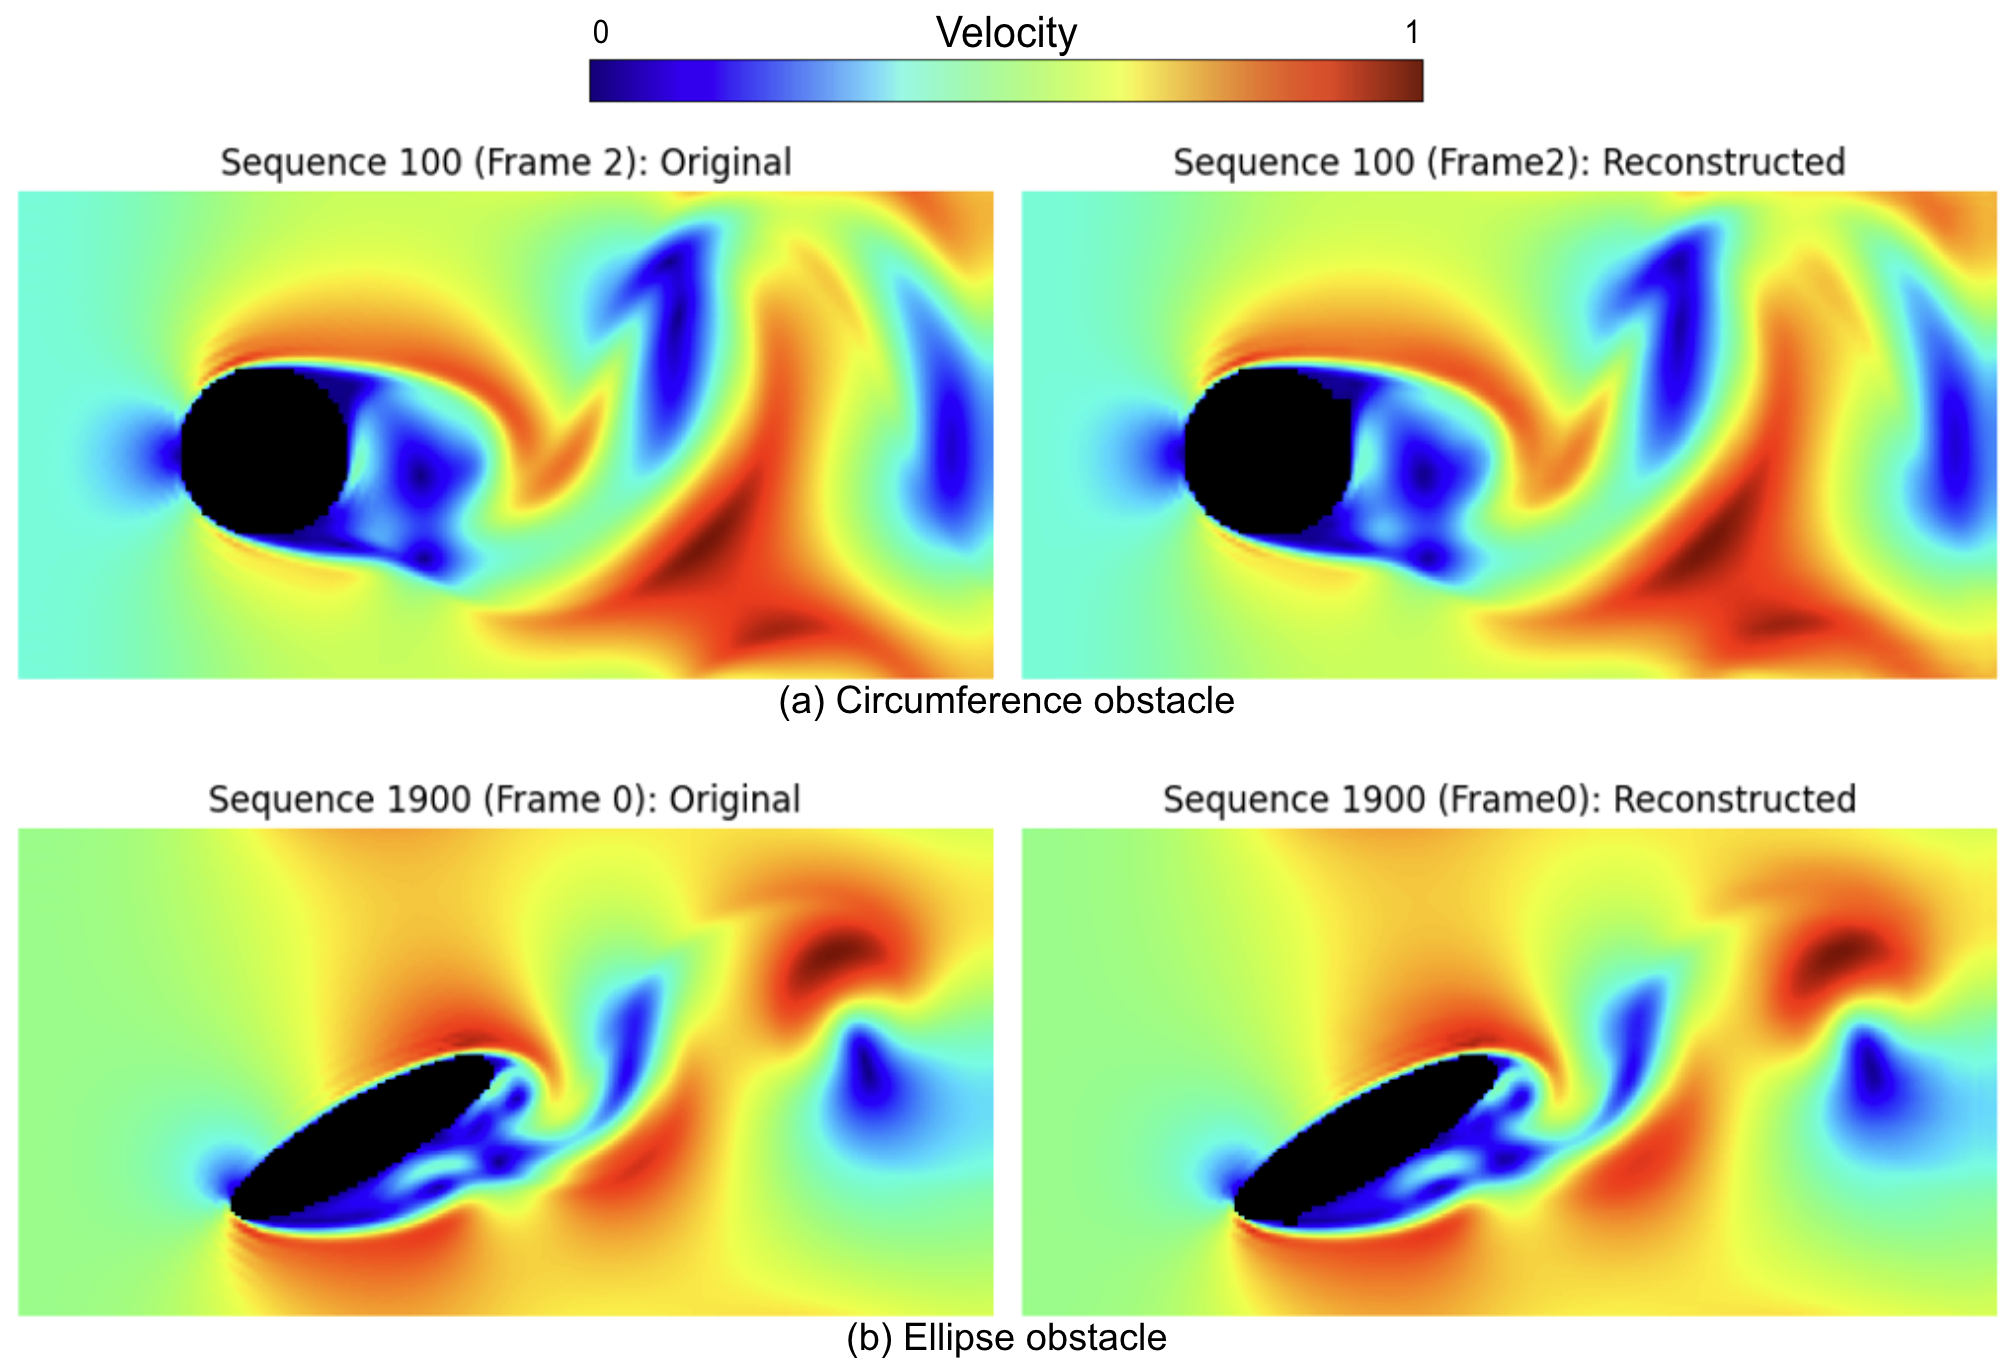
\includegraphics[width=1\linewidth]{images/autoencoder_frames.png}
    \caption{Original vs Reconstructed frames}
    \label{fig:ReconstructedFrames}
\end{figure}

For the following evaluation method, we compare the velocity values between the Original and Reconstructed frames to verify their similarity. This is done by creating a histogram of velocities, i.e., a frequency count of velocity values on each grid cell in the frame. Figure~\ref{fig:ReconstructedHistograms} shows examples of those histograms for Origianl and Reconstructed frames containing each type of obstacle. The frame examples are the same as Figure~\ref{fig:ReconstructedFrames} used in the previous evaluation method. On the x-axis, we have the range of all the velocity values in the frame. These values are between 0 and 1 because the data was previously normalized, as explained in Section~\ref{sec:DataPreparation}. On the y-axis, the frequency or occurrence of each velocity value is represented. To compare all the velocity histograms, we calculated the Jensen-Shannon distance between each frequency distribution. The resulting average distance between the original and reconstructed frames was 0.021, with a standard deviation of 0.014.

% In the example shown, we can see a lot of coincidence between the corresponding histogram bars of each frame. Similarly to the previous evaluation, we can see some differences between the histogram bars, but nothing significant. Some of the bars are taller or shorter, coinciding with the color intensity difference observed in the \textit{heatmaps} of the previous evaluation. Similar results were observed on the histograms of other sequences.

\begin{figure}[H]
    \centering
    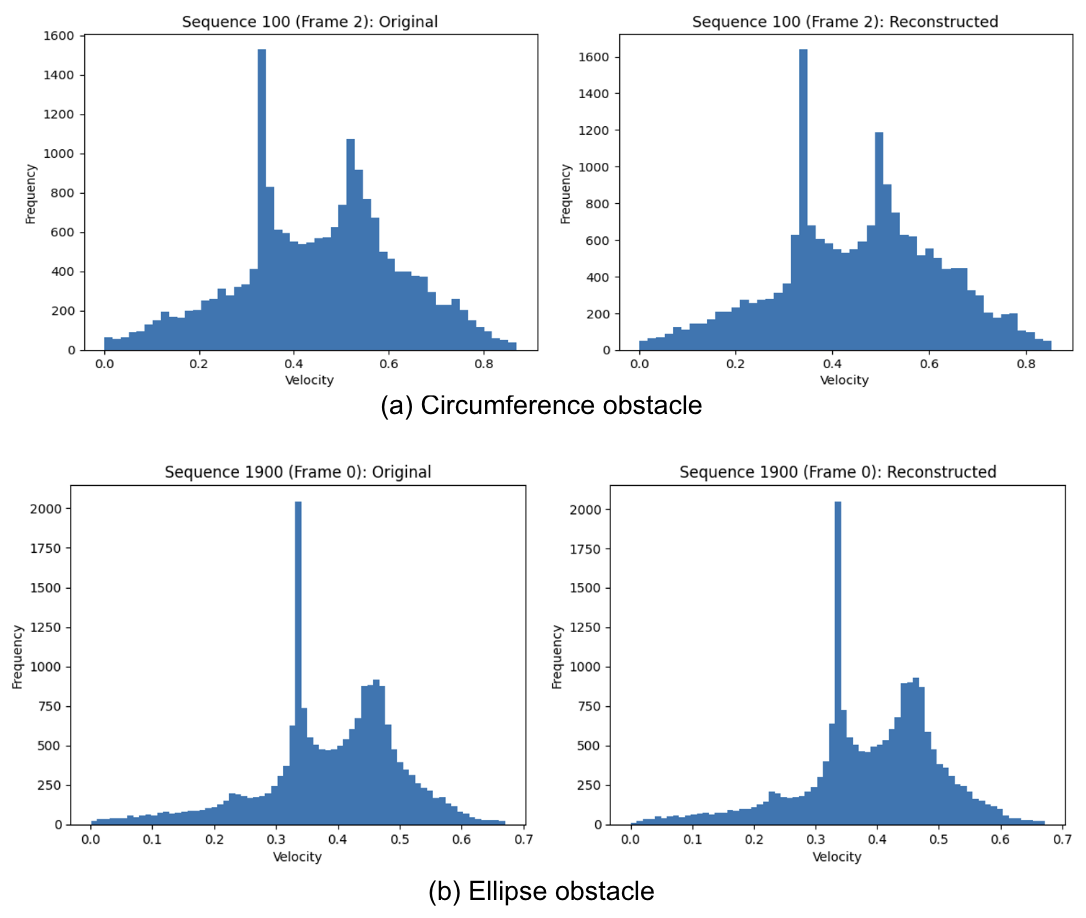
\includegraphics[width=1\linewidth]{images/autoencoder_histogram.png}
    \caption{Original vs Reconstructed frames velocity histograms}
    \label{fig:ReconstructedHistograms}
\end{figure}

Both evaluations tell us that the Autoencoder successfully reduces the data's dimensionality so that the original data can be reconstructed using that low-resolution representation. This means that the training of this model's component was successful. Although there are some minor errors, the fluid flow structure remains correct, and the approximations of the velocities are very close.

The Autoencoder is a vital component of the model because it guarantees that the model successfully extracts enough information to represent the original data. This process of reducing the amount of information with a lower representation is important to support the next phase, which is the generation of the next fluid state.

%----------------------
\section{Generator Results}
\label{sec:GeneratorResults}
%----------------------

The Generator's goal is to generate the next fluid flow state using as an input the low-resolution representation created by the Encoder. To evaluate this component, the resulting frame is compared against the expected frame taken from the dataset created by the numerical simulation. For this evaluation we used similar methods than the Autoencoder evaluation.

Figure~\ref{fig:GeneratedFrames} shows a comparison between a generated frame velocity \textit{heatmap} at the right, and the expected frame at the left. The images show a result example for each of the possible obstacle types. Similar to the Autoencoder results, very small differences appear in the \textit{heatmap} colors, however, both images are almost similar.

We created the velocity histogram for each generated frame and compared it to the original frame. Figure~\ref{fig:GeneratedHistograms} compares 2 examples of the velocity histograms. Then, we calculated the Jensen-Shannon distance between the velocity distributions of the frames in all the sequences. This results in an average distance between the expected and generated frames of 0.043 with a standard deviation of 0.010. The low average value of the distance metric between both distributions indicates that the original and generated frames are very similar.

\begin{figure}[!htbp]
    \centering
    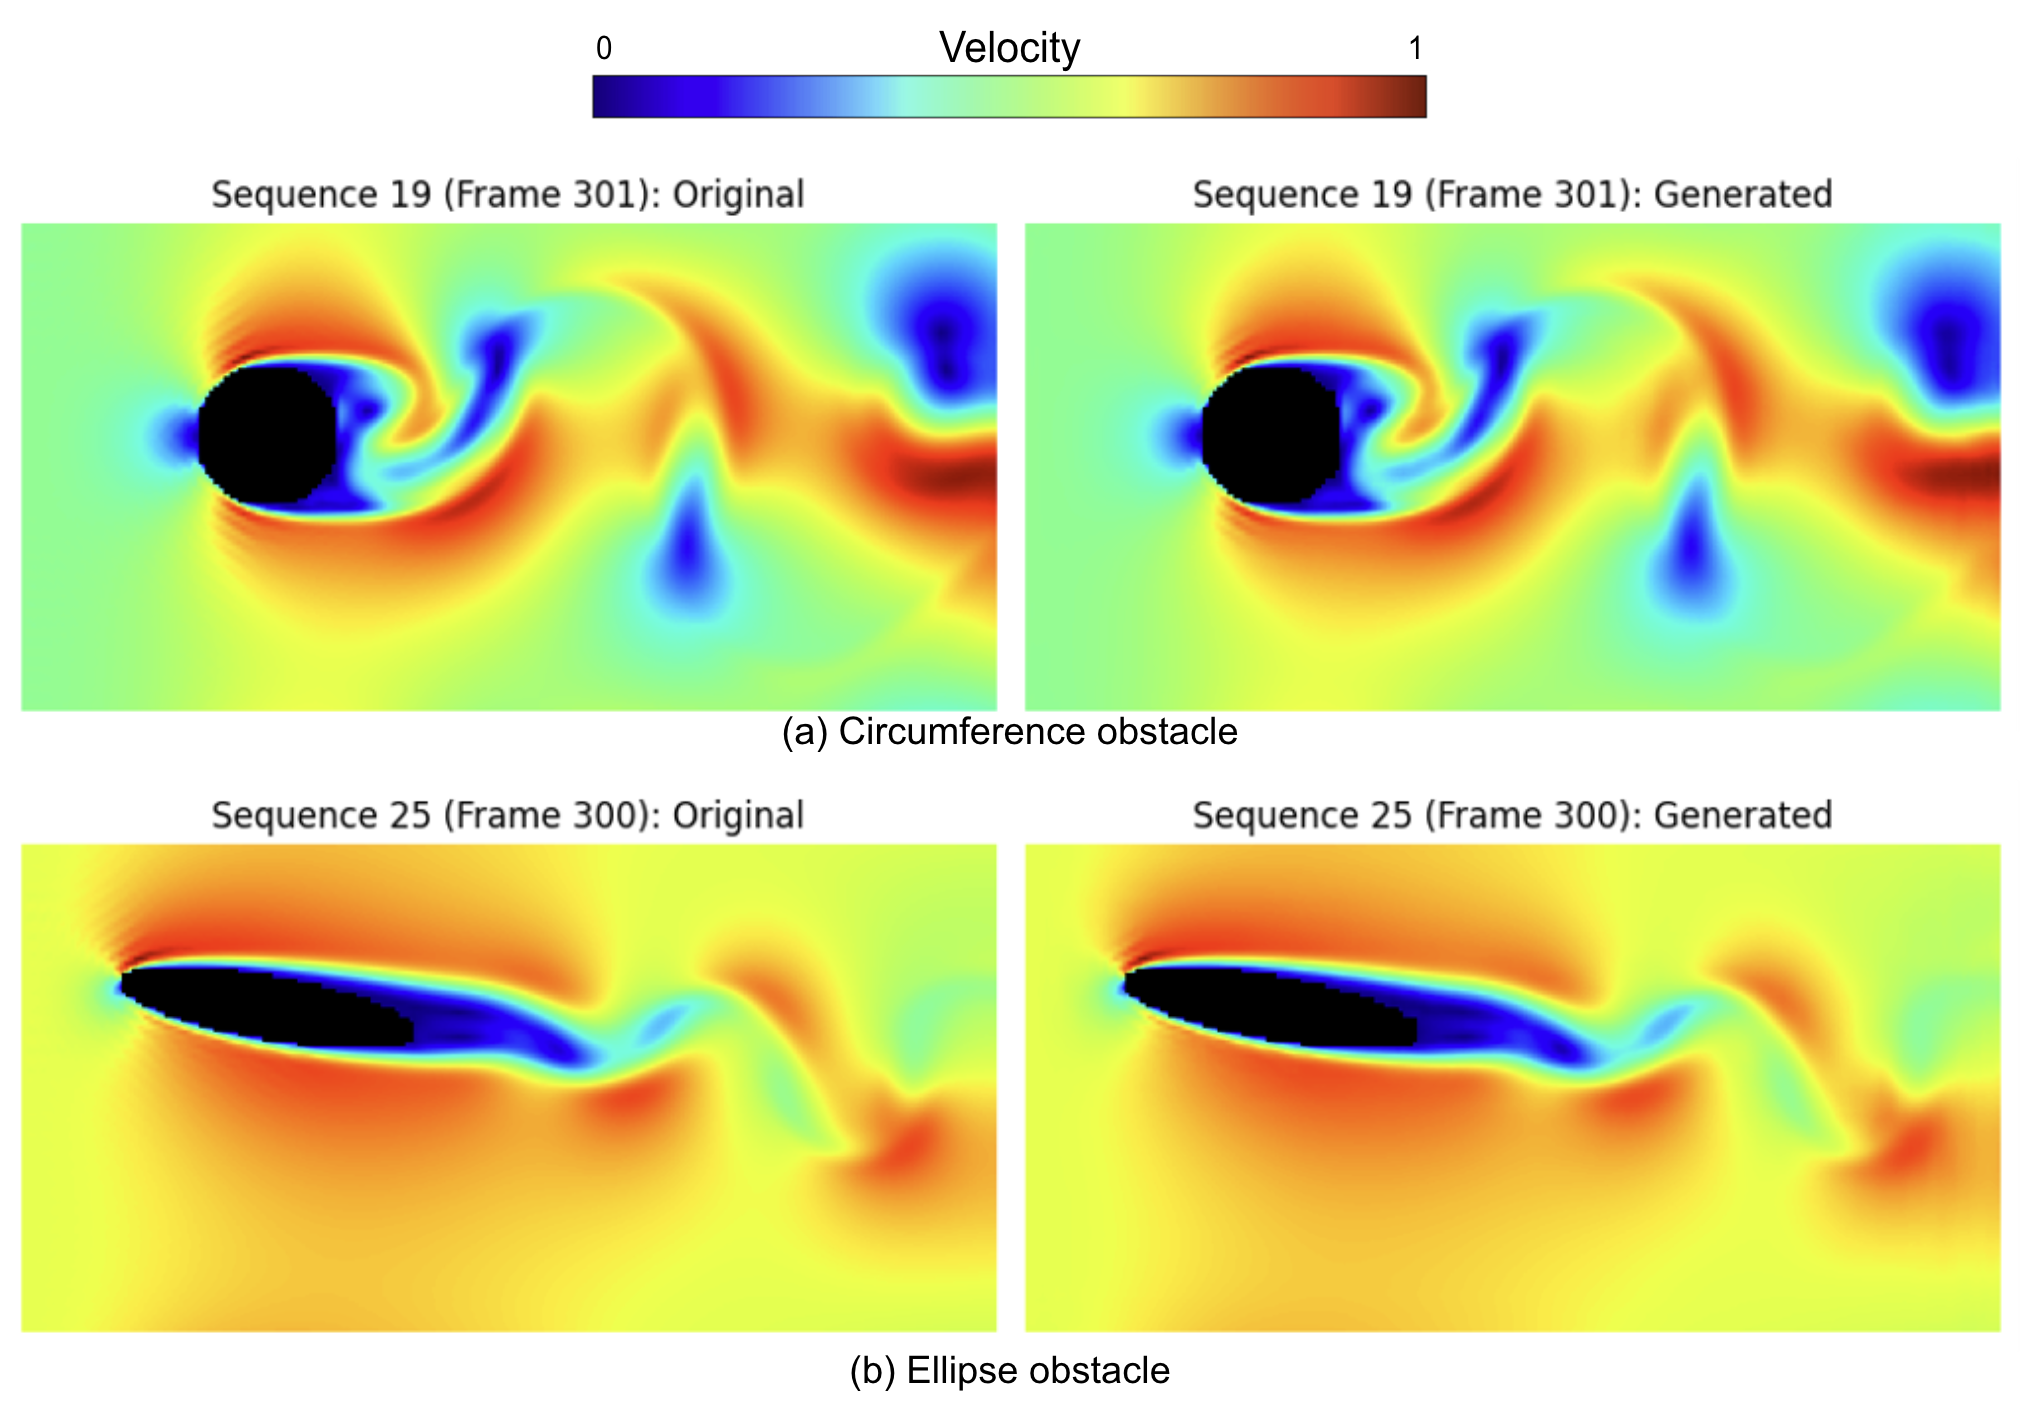
\includegraphics[width=1\linewidth]{images/generator_frames.png}
    \caption{Original vs Generated frames}
    \label{fig:GeneratedFrames}
\end{figure}

\begin{figure}[!htbp]
    \centering
    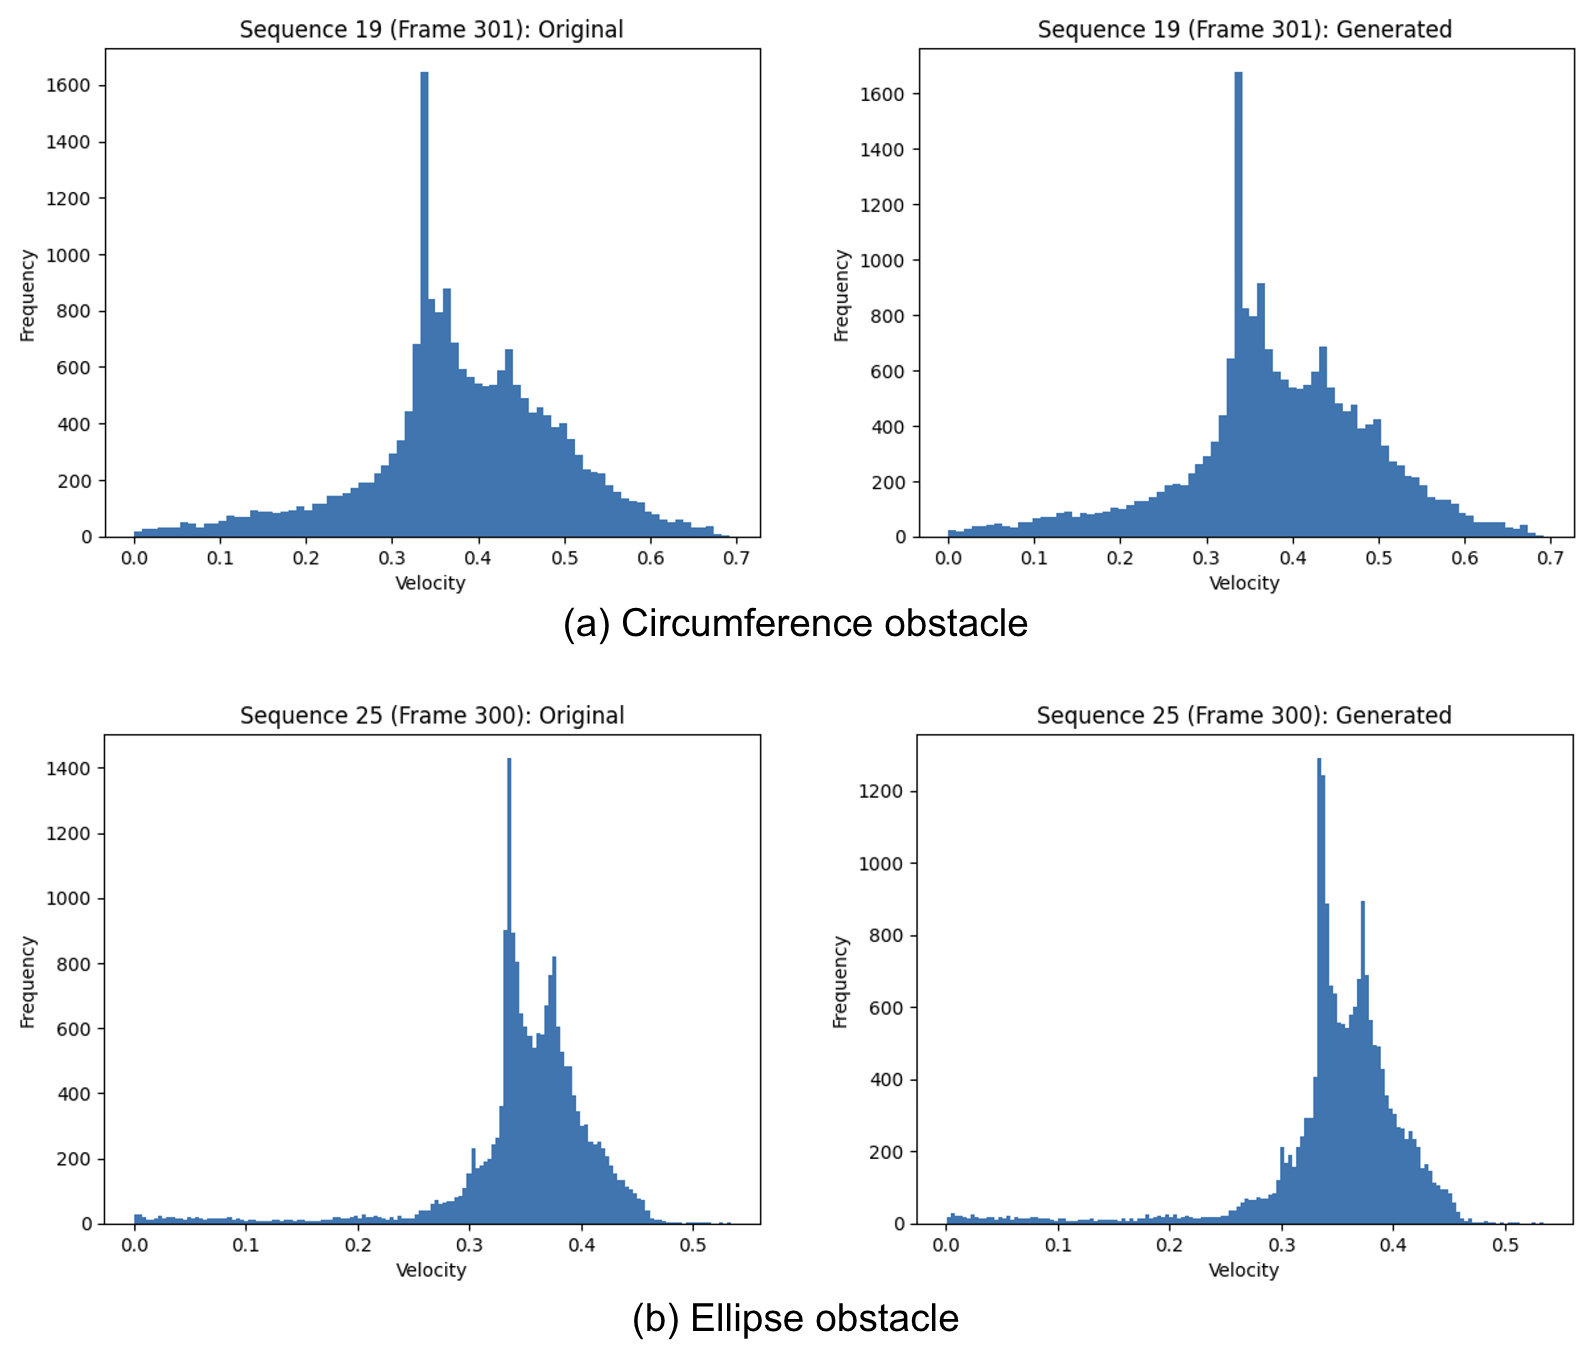
\includegraphics[width=1\linewidth]{images/generated_histogram.png}
    \caption{Original vs Generated frames velocity histograms}
    \label{fig:GeneratedHistograms}
\end{figure}


These evaluations show that the model can successfully approximate the next state in the fluid flow sequence. The same level of accuracy in both evaluation methods was observed across all the cases in the testing dataset. Although there are some differences between the expected and generated frames, the model can replicate the evolution of the fluid flow structure across the sequence simulation time.

%----------------------
\section{Model Performance}
\label{sec:ModelPerformance}
%----------------------

In this section we explore the results of the two main metrics chosen to evaluate this models performance as explained in Section~\ref{sec:ResearchObjectiveandSolution}. These metrics are: the Error measured with MSE, and the execution time of the simulation measured in seconds.

\subsection{Error Measurements}
\label{subsec:ErrorMeasurements}

Figure~\ref{fig:ErrorMeasurements} shows the results of the MSE metric. The results are divided into three groups, one for all the shapes in the dataset together, one with only Circumferences obstacles, and another for Ellipses obstacles. The minimum, maximum, and average error values are plotted for each group. It is important to mention that the dataset is balanced, meaning that the amount of examples with each obstacle type is the same, which is essential to ensure fairness in the results. 

The following analysis can be done by looking at the MSE plots in Figure~\ref{fig:ErrorMeasurements}. We can see that the minimum and maximum errors across the entire dataset are both in simulations with an ellipse obstacle. Additionally, the difference between the minimum and maximum error is lower for the circumference than the ellipse obstacle. This could be caused by circumference obstacles presenting less variability in their shapes, with only a change in the radius, while ellipses obstacles have more diversity in their shapes. This variability in the obstacle shapes makes it more challenging for the model to learn how to simulate the ellipse objects. However, because the average errors are similar between the two types of obstacles, we can conclude that no specific obstacle shape is significantly more difficult for the model to simulate. 

\begin{figure}[!htbp]
    \centering
    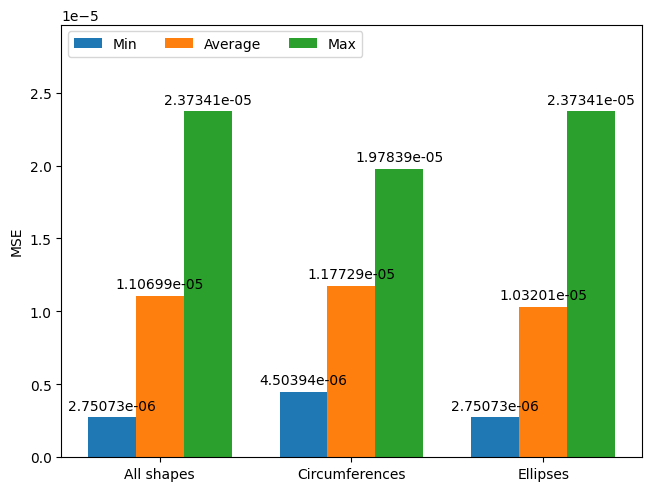
\includegraphics[width=0.7\linewidth]{images/MSE.png}
    \caption{Model MSE error metric}
    \label{fig:ErrorMeasurements}
\end{figure}


\subsection{Execution time}
\label{subsec:ExecutionTime}
As explained in Section~\ref{sec:ResearchObjectiveandSolution}, the goal of this model is to reduce the execution time of the simulation while maintaining a low error to preserve the pattern structure of the fluid flow in the generated sequence. Table~ \ref{tab:ExecutionTime} compares execution time between the simulation and the DL Model. The simulation took, on average, 191 seconds (3.2 minutes), while the DL model took, on average, only 42 seconds. This represents a 4.5 times improvement in execution speed over the numerical simulation. This result shows that using this DL model improves the simulation's performance, reducing the total execution time while successfully simulating the evolution of the fluid flow. 


% \begin{figure}[!htbp]
%     \centering
%     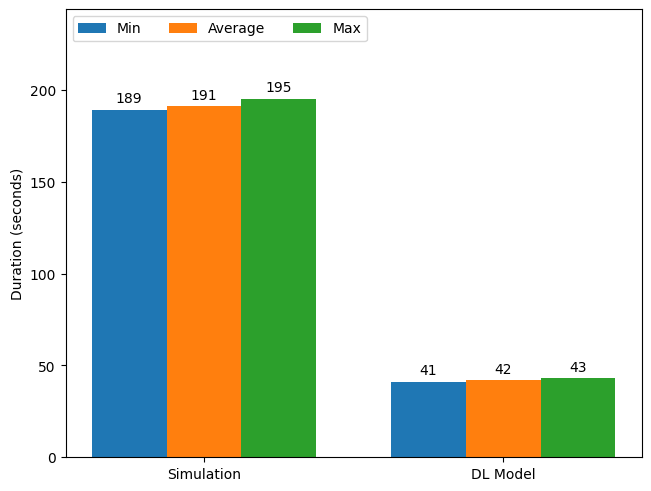
\includegraphics[width=0.7\linewidth]{images/execution_time.png}
%     \caption{Model execution time}
%     \label{fig:ExecutionTime}
% \end{figure}


\begin{table}[ht]
    \caption{CFD simulation vs DL Model execution time}
    \centering
    \begin{tabular}{|c|c|}
    \hline
                    & Average Execution Time \\ \hline
    CFD Simulation  & 191 \\ \hline
    DL Model        & 42 \\ \hline
    \end{tabular}
    \label{tab:ExecutionTime}
\end{table}



% ============================================================
%
%                   CHAPTER 6: CONCLUSION
%
% =============================================================

\chapter{Conclusion}
\label{ch:Conclusion}

% % --------------------------------------
\section{Takeaways}
\label{sec:Takeaways}
% % --------------------------------------
The following are the key takeaways of this project:
\begin{enumerate}[label=\alph*.]
\item Apple Neural Engine (ANE) Utilization: This project explored leveraging the underused NPU for LLM inference, going beyond standard CoreML use cases and showed that it can be viable.

\item Retrieval-Augmented Generation (RAG) without Internet : Implements a lightweight RAG pipeline that only uses on device resources.

\item Portability and Ease of use: Application size of less than 1GB that includes everything, available for download at \href{https://tldr.cool}{\textbf{https://tldr.cool}}

\item Quantized LLMs: Uses compact models (50–500MB) for efficient, on-device inference allowing for seamless multitasking and manages to obtain results comparable to mainstream cloud LLMs.
\end{enumerate}
% % --------------------------------------
\section{Limitations}
\label{sec:Limitations}
% % --------------------------------------
Following are the main limitations uncovered during the implementation of this project:
\begin{enumerate}[label=\alph*.]
\item While this project demonstrates the feasibility to accelerate the retrieval part of the RAG pipeline, the LLM Inference still only leverages the GPU and does not leverage the NPU.

\item Indexing(embedding) takes 90+% of overall runtime

\item Many smaller LLMs available currently (3B or less) are only instruction-tuned i.e trained for text completion and not for chat. This can lead to unfavorable responses during chat.

\item Excessive usage limits to quick draining of power, especially on portable devices.

\item The breadth of retrieval space is limited not by resources but by the context size of the Chat LLM, since both input and expected output must fit in the LLM context.

\end{enumerate}
% % --------------------------------------
\section{Future work}
\label{sec:FutureWork}
% % --------------------------------------
\begin{enumerate}[label=\alph*.]
    \item Enhance data safety mechanisms for vectordump files.
    \item Add NPU backend for GGML and llama.cpp.
    \item Quantize and convert fine-tuned chat-optimized LLMs to the GGUF format.
    \item Implement a dedicated parallelized tokenization module.
    \item Extend the application support beyond Apple Silicon.
    \item Add NPU and GPU acceleration support for SQLite and Postgres vector search extensions (they currently only support CPU).
    \item Create an optimized decoding and tokenization workflow dedicated for embedding (e.g., no KV cache).
\end{enumerate}

\printendnotes

%
% ==========   Bibliography
%
% \nocite{*}   % include everything in the uwthesis.bib file
\bibliographystyle{unsrt}
\bibliography{uwthesis}
%
% ==========   Appendices
%

\end{document}